\documentclass[a4paper,10pt]{article}

%%%%%%%%%%%%%%%%%%%%%%%%%%%%%%%%%%%%%%%%%%%%%%%%%%
% Los paquetes permiten ampliar las capacidades de LaTeX.                     %
%%%%%%%%%%%%%%%%%%%%%%%%%%%%%%%%%%%%%%%%%%%%%%%%%%
% Paquete para inclusión de gráficos.
\usepackage{graphicx}

% Paquete para definir la codificación del conjunto de caracteres usado
\usepackage[utf8x]{inputenc}

% Paquete para definir el idioma usado.
\usepackage[spanish]{babel}

% Paquete para introducir codigo de programacion
\usepackage{listings}

 % Para poder introducir otrod PDFs
\usepackage{pdfpages}

% Para inseratar imagenes
\usepackage{graphicx}
\usepackage{subcaption}
\usepackage{float}
\usepackage{longtable}


%Para encabezado y pie de pagina
\usepackage{fancyhdr}

%Para margenes
\usepackage{vmargin}

%Ecuaciones
\usepackage{amssymb, amsmath, amsbsy} % simbolitos
\usepackage{upgreek} % para poner letras griegas sin cursiva
\usepackage{cancel} % para tachar
\usepackage{mathdots} % para el comando \iddots
\usepackage{mathrsfs} % para formato de letra
\usepackage{stackrel} % para el comando \stackbin

\setpapersize{A4}
\setmargins{1.5cm}       % margen izquierdo
{1.5cm}                        % margen superior
{16.5cm}                      % anchura del texto
{23.42cm}                    % altura del texto
{10pt}                           % altura de los encabezados
{1cm}                           % espacio entre el texto y los encabezados
{0pt}                             % altura del pie de página
{2cm}                           % espacio entre el texto y el pie de página

\usepackage{cleveref}

\begin{document}

\pagestyle{fancy}
\fancyhf{}
\lhead{\begin{picture}(0,0) \put(0,0)
{
\includegraphics[width=30mm]{./Logo2.jpg}} \end{picture}}

\fancyhead[R]{66.69 Criptografia y Seguridad Informatica}
\fancyfoot[R]{\thepage}


% Título principal del documento.
\title{\textbf{Trabajo Practico final: Deteccion de anomalias con Machine Learning}}



% Información sobre los autores.
\author{Agustin Miguel Payaslian (\#96.885)\\
\texttt{agustin.payaslian@gmail.com}\\
\\
Augusto Arturi (\#97498)\\
\texttt{turitoh@gmail.com}\\
\\
Estanislao Ledesma (\#96622)\\
\texttt{estanislaomledesma@gmail.com}\\
\\
\vspace{5mm}
\normalsize{2do. Cuatrimestre de 2018}\\
\vspace{5mm}
\normalsize{66.69 Criptografia y Seguridad Informatica}\\
\vspace{5mm}
\normalsize{Facultad de Ingeniería, Universidad de Buenos Aires}\\
}
\date{}


% Inserta el título.
\maketitle

\vspace{5mm}
\begin{figure}[!htp]
\centering

\includegraphics[scale=1]{Logo.png} 
\end{figure}
\vspace{5mm}

% Quita el número en la primer página.
\thispagestyle{empty}


\newpage

\tableofcontents

\newpage


\begin{abstract}
	En el siguiente trabajo practico se explicaran mediantes dos casos practicos la utilizacion de algoritmos y metodologias de machine learning aplicadas a problemas de la seguridad informatica.
\end{abstract}  

\newpage

\section{Introduccion}

Se cree que las tecnologías de Machine Learning pueden aportar mucho valor al mundo de la seguridad. Una de las aplicaciones directas conocidas de estas técnicas es la \textbf{detección de anomalías de tráfico de red}. Esta hace referencia a comportamientos no esperables de acuerdo al funcionamiento habitual de la red. Por ejemplo, situaciones en las que se genere gran cantidad de tráfico repentino o muy diferente al habitual. El arte de estas técnicas consiste precisamente en determinar qué es diferente, habitual y disponer de los mecanismos adecuados para detectarlo. 

\subsection{Random Forest}
Es un algoritmo de Machine Learning de aprendizaje supervisado. Es una combinación de árboles predictores tal que cada árbol depende de los valores de un vector aleatorio probado independientemente y con la misma distribución para cada uno de estos. Se caracteriza por:
\begin{itemize}
\item Ser uno de los algoritmos de aprendizaje más certeros que hay disponible. Para un set de datos lo suficientemente grande produce un clasificador muy certero. 
\item Correr eficientemente en bases de datos grandes.
\item Manejar cientos de variables de entrada sin excluir ninguna.
\item Dar estimaciones de qué variables son importantes en la clasificación.
\item Tener un método eficaz para estimar datos perdidos y mantener la exactitud cuando una gran proporción de los datos está perdida.
\item Sirve tanto para problemas de clasificación como de regresion
\item Computar las proximidades entre los pares de casos que pueden usarse en los grupos, localizando valores atípicos, o (ascendiendo) dando vistas interesantes de los datos.
\item Ofrecer un método experimental para detectar las interacciones de las variables.
\end{itemize}


\textbf{Bagging} en general implica aplicar el mismo clasificador n veces y luego promediar sus resultados para el obtener el resultado final. El problema es que aplicar el mismo clasificador n veces al mismo set de datos dara n veces el mismo resultado. Es por esto que bagging siempre se usa en conjunto con bootstrapping. \\

\textbf{Bootstrapping} consiste en tomar una muestra del set de entrenamiento del mismo tamaño del set de entrenamiento pero con reemplazo. Es decir que un dato puede estar varias veces en la muestra. Como cada clasificador no ve el total de registros del set de entrenamiento la técnica de bagging disminuye notablemente las posibilidades de caer en overfitting, ya que ninguno de los n clasificadores individuales puede sobreajustar al set de entrenamiento completo.

Bagging puede usarse con cualquier algoritmo de clasificación o regresión pero es muy popular con árboles de decisión, en donde da origen al algoritmo de Random Forests, el cual es uno de los algoritmos más populares en clasificación porque suele predecir buenos resultados para la mayoría de los set de datos, lo cual hemos comprobado a lo largo de este trabajo práctico.

\medskip

En definitiva un RF es un conjunto de árboles de decisión en donde cada árbol usa un bootstrap del set de entrenamiento y un cierto conjunto de atributos tomados al azar. Los RF tienen, en general, dos hiper parámetros: la cantidad de árboles a crear y la cantidad de atributos de cada uno. 

El primero (cantidad de árboles) no es muy complejo ya que en general a mayor cantidad de árboles mejor funciona el ensamble pero hay que tener en cuenta que llegado un punto la mejora es prácticamente inapreciable y perdemos performance, por esto en general usaremos una cantidad de árboles que podamos manejar y que nos den el mejor resultado posible o bien que no tengan una diferencia apreciable con el uso de mayor cantidad de árboles.

\begin{figure}[!htp]
\centering
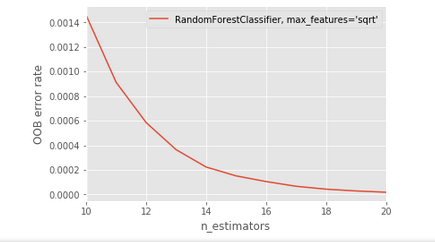
\includegraphics[scale=0.6]{Wireshark/OOB_1.png} 
\caption{}
\end{figure}

En la figura 5  observamos cómo a partir de los 20 árboles el error se va prácticamente a cero y la mejora a más árboles es inapreciable.

El segundo hiper-parámetro: la cantidad de atributos por árbol es el mas critico y necesita ser encontrado mediante la toma de subconjuntos de atributos tomados al azar lo cual ayuda a determinar cuales son los atributos que realmente importan para la clasificación promediando su precisión. 

\section{Primer caso}
En este primer ejemplo práctico se utilizo el dataset \textbf{KDD99}. Este dataset fue creado para el “Third International Knowledge Discovery and Data Mining Tools Competition”.El objetivo de esta competencia era construir un detector de intrusiones de la red (network intrusion detector), es decir un modelo predictivo que sea capaz de distinguir entre conexiones “malas” y conexiones ”buenas”. Este contiene una gran cantidad de tráfico , dentro del cual se encuentran intrusiones simuladas en un ambiente de red militar.
Cada conexión tiene una categoría, ya sea normal, o el nombre específico del ataque.\\


Los ataques se encuentran dentro de estas categorías:


\begin{itemize}
\item DOS:     denegacion de servicio (Denial Of Service)

\item R2L: acceso no autorizado desde un usuario remoto.

\item U2R:  acceso no autorizado a privilegios de superusuario.

\item probing: vigilancia y otro tipo de sondeos. Ej: escaneo de puertos


\subsection{Analisis exploratorio}


Este dataset esta dividido en 2 archivos. El archivo “10perfect” es el que se utiliza para obtener la informacion para entrenar el algoritmo y el archivo “corrected” que es el que se utiliza para verificar la precision de la prediccion.

Este provee informacion de valor por medio de sus features, los cuales seran trabajados como parte del preprocesado para luego entrenar al algoritmo deseado. La informacion basica provista por el mismo es la siguiente:


\begin{center}
\begin{longtable}{|l|l|}

\hline
Feature name & Description  \\
\hline
duration  & length (number of seconds) of the connection   \\
protocol\_type &
type of the protocol, e.g. tcp, udp, etc \\
service 
& network service on the destination, e.g., http, telnet, etc. \\
src\_bytes 
& number of data bytes from source to destination \\

dst\_bytes 
& number of data bytes from destination to source 
\\

flag 
& normal or error status of the connection 
\\

land 
& 1 if connection is from/to the same host/port; 0 otherwise 
\\

wrong\_fragment 
& number of ``wrong'' fragments \\
urgent 
& number of urgent packets \\
hot 
& number of ``hot'' indicators \\
num\_failed\_logins 
& number of failed login attempts  \\
logged\_in 
& 1 if successfully logged in; 0 otherwise  \\
num\_compromised 
& number of ``compromised'' conditions  \\
root\_shell 
& 1 if root shell is obtained; 0 otherwise  \\
su\_attempted 
& 1 if ``su root'' command attempted; 0 otherwise  \\
num\_root 
& number of ``root'' accesses  \\
num\_file\_creations 
& number of file creation operations  \\
num\_shells 
& number of shell prompts  \\
num\_access\_files 
& number of operations on access control files  \\
num\_outbound\_cmds
& number of outbound commands in an ftp session  \\
wrong\_fragment 
& number of ``wrong'' fragments \\
is\_hot\_login 
& 1 if the login belongs to the ``hot'' list; 0 otherwise \\
is\_guest\_login 
& 1 if the login is a ``guest''login; 0 otherwise \\
count 
& number of connections to the same host as the current connection in the past two seconds \\
serror\_rate 
& \% of connections that have ``SYN'' errors \\
rerror\_rate 
& \% of connections that have ``REJ'' errors \\
same\_srv\_rate 
& \% of connections to the same service \\
diff\_srv\_rate 
& \% of connections to different services \\
srv\_count 
& number of connections to the same service as the current connection in the past two seconds \\
srv\_serror\_rate 
& \% of connections that have ``SYN'' errors \\
srv\_rerror\_rate 
& \% of connections that have ``REJ'' errors \\
srv\_diff\_host\_rate 
& \% of connections to different hosts \\

\hline

\end{longtable}
\label{tabla:sencilla}
\end{center}



\end{itemize}


El feature \textbf{label} corresponde al tipo de ataque al que pertenece el trafico y es uno de los mas importantes del set de datos, ya que este valor es el cual queremos clasificar.

En la Figura 1 se observa todos los tipos de ataques junto con su respectiva cantidad de apariciones.


\medskip
\begin{figure}[!htp]
\centering
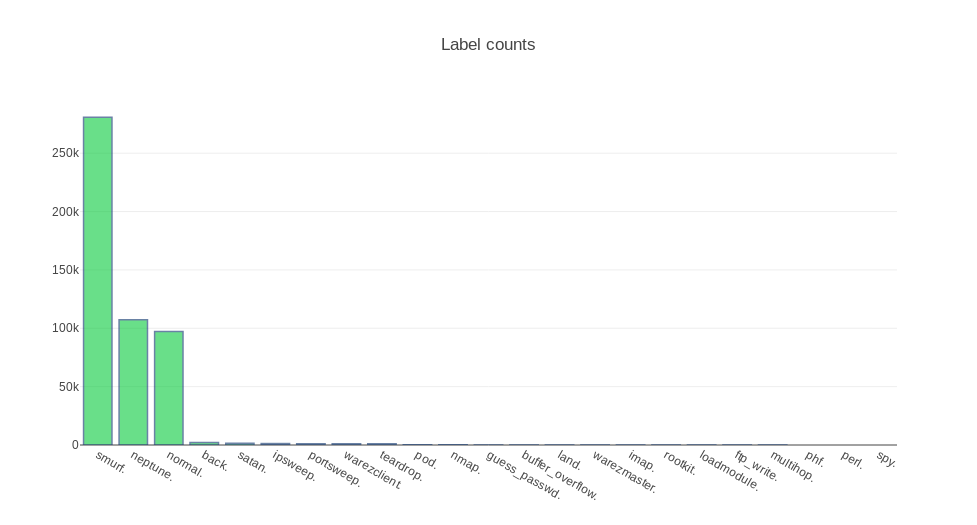
\includegraphics[scale=0.5]{Wireshark/newplot.png} 
\caption{}
\end{figure}

Para una mejor categorizacion, los ataques fueron agrupados por las 4 categorias mencionadas anteriormente

\newpage
\medskip
\begin{figure}[!htp]
\centering
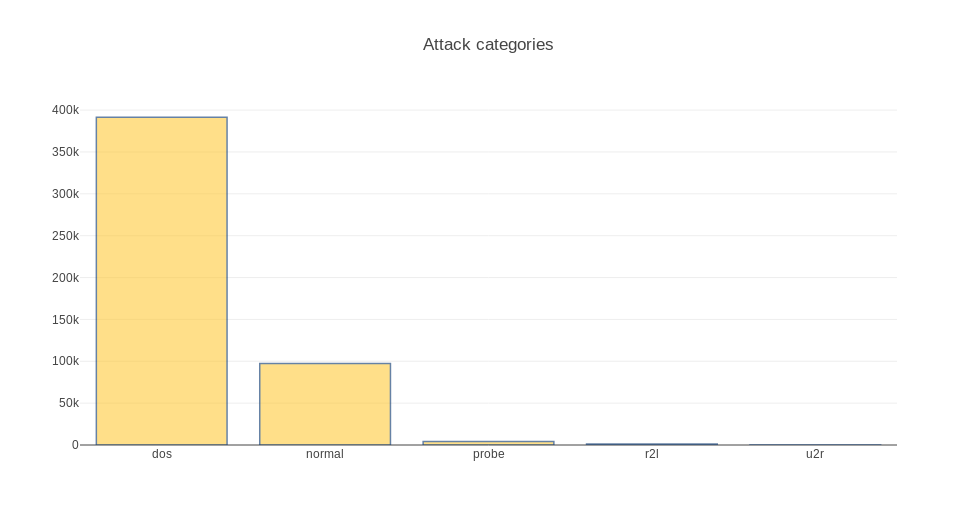
\includegraphics[scale=0.5]{Wireshark/newplot(1).png} 
\caption{}
\end{figure}


La solucion que se plantea en este primer caso implica analizar  el tráfico que pertenece a ataques de DOS y el tráfico normal. 
\medskip
\begin{figure}[!htp]
\centering
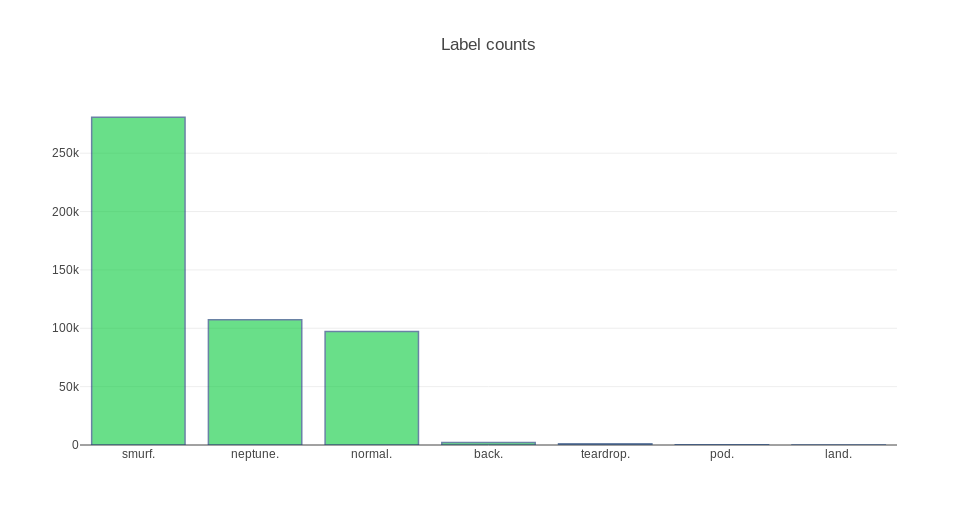
\includegraphics[scale=0.5]{Wireshark/newplot(2).png} 
\caption{}
\end{figure}

.
\newpage
\lstset{language=Python}
\lstset{frame=lines}
\lstset{caption={De todas formas, las filas eliminadas solo representan un 1\% del set de datos}}
\lstset{label={lst:code_direct}}
\lstset{basicstyle=\footnotesize}
\begin{lstlisting}
1.0 - len(dfAnalysis.loc[(dfAnalysis.cat_attack == "dos") | 
 (dfAnalysis.cat_attack == "normal")]) /len(dfAnalysis)


Out: 0.01069792579667661
\end{lstlisting}

Finalmente para terminar el preprocesado se acomodo la informacion de una forma tal que le sea mas util a nuestro algoritmo para eso usamos funciones de normalizacion de los datos y funciones de \textit{one hot encoding} la cual consiste endividir el atributo en tantas columnas como valores posibles puede tener y usar cada columna como un dato binario indicando si el atributo toma o no dicho valor.

\subsection{Entrenamiento}
Se trabajo con un set de entrenamiento y un set de test. La
idea consisten en entrenar a nuestro algoritmo con el set de entrenamiento y
luego lo aplicaremos al set de test. De esta forma, los datos para los cuales
queremos probar el algoritmo nunca fueron vistos por el mismo, lo cual permite
saber si el modelo fue capaz de generalizar correctamente. Para poder validar
el modelo necesitamos dividir el set de entrenamiento original en dos: un set de
entrenamiento y un set de validación. La idea es entrenar el modelo con el set
de entrenamiento y luego probarlo con el set de validación a efectos de encontrar
los mejores hiper-parámetros pertenecientes propios a cada algoritmo. El set de validación utilizado fue de un 25\% del set de entrenamiento.\\


Utilizamos el algoritmo de \textbf{random forest} para realizar la predicción. Para ello con la información obtenida del archivo “10perfect” entrenamos el algoritmo y luego predecimos los ataques para el archivo “corrected”. Para verificar la eficacia del algoritmo comparamos los valores obtenidos obtenidos por la predicción con los que ya se encontraban en el archivo. Al realizar la comparación obtuvimos el resultado siguiente:

\textbf{Accuracy: 0.9946986695597958}


\medskip

\normalsize Es decir el algoritmo diferenció con una precisión del 99\% el trafico normal, del que se trataba de un ataque DOS.


Los features que mas importaron a la hora de la prediccion fueron los siguientes:
\begin{figure}[!hbp]
\centering
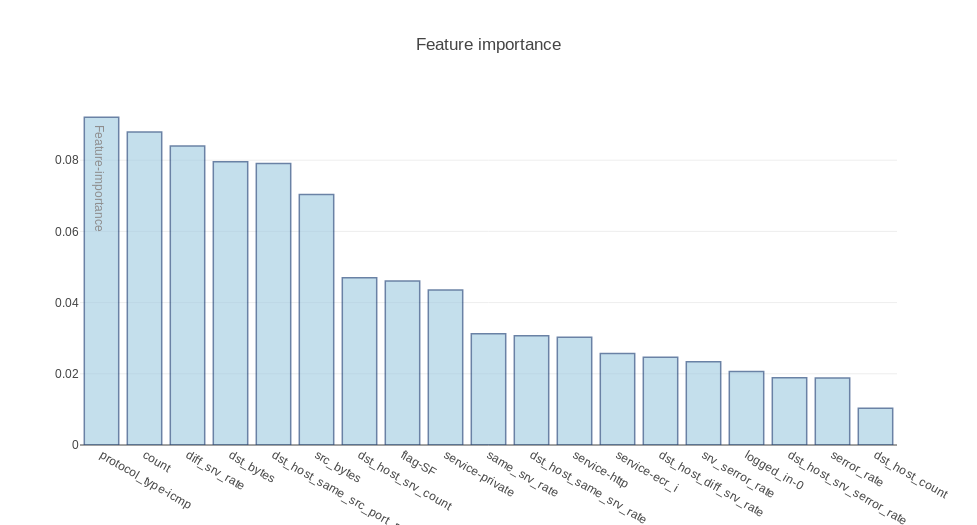
\includegraphics[scale=0.4]{Wireshark/newplot(5).png} 
\caption{}
\end{figure}

Es decir, que a partir de la figura anterior se puede interpretar que features aportan mas valor para generar el arbol de decision que clasifique al random forest.



\newpage
\section{Segundo caso}


En este segundo ejemplo práctico, se decidió trabajar sobre otro dataset, esta vez con un enfoque más realista el cual implica realizar un estudio previo de los datos y el problema para luego entrenar al algoritmo.

\medskip
En primer lugar se tomo un ejemplo del sitio web \textsuperscript{[1]} este resulto de gran interés ya que aquí se suben archivos de tráfico de red con malware, en el cual quien analiza el mismo debe encontrar en qué lugares existe una anomalía.

\subsection{Estudio del trafico}

A continuación se explica como fue estudiado el tráfico de red de este problema con la herramienta Wireshark.

\begin{figure}[!htp]
\centering
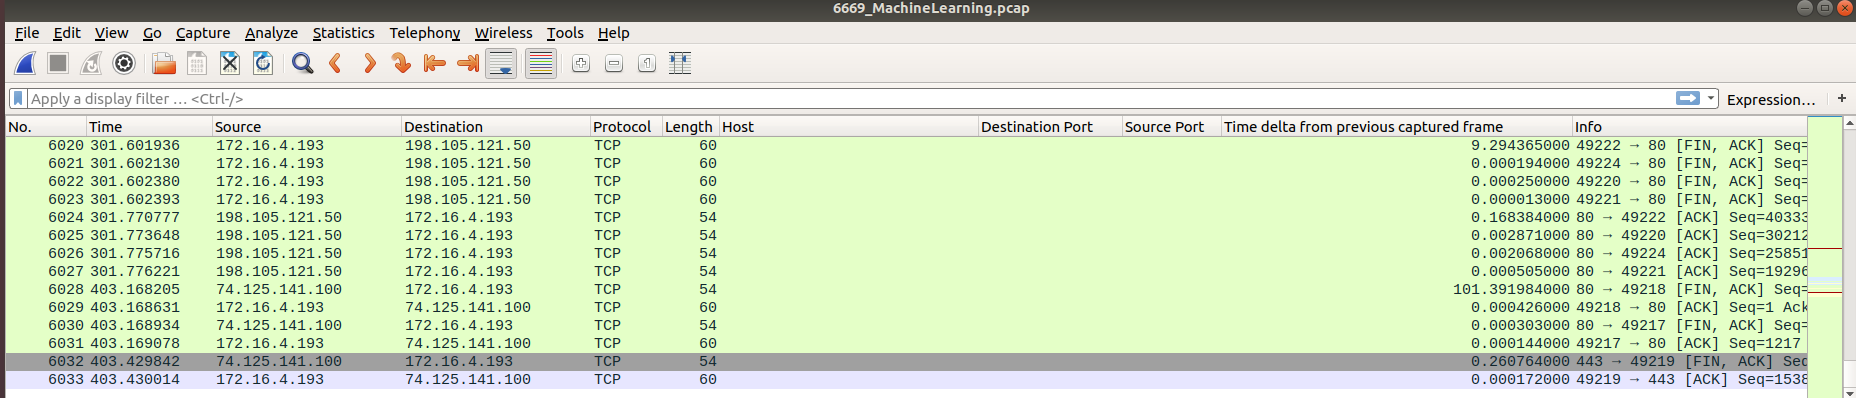
\includegraphics[scale=0.2]{Wireshark/1.png} 
\caption{}
\end{figure}

En la figura simplemente se observa la cantidad de paquetes que se intercambio durante la toma de trafico, siendo esta 6033, como medida de dificultad para entender a que problema uno se enfrenta.
Luego se utiliza el filtro \textbf{http.request} para verificar a que host se comunicó el cliente durante toda la conexión

%%%%%%%%%
\newpage
%%%%%%%%%

\medskip
\begin{figure}[!htp]
\centering
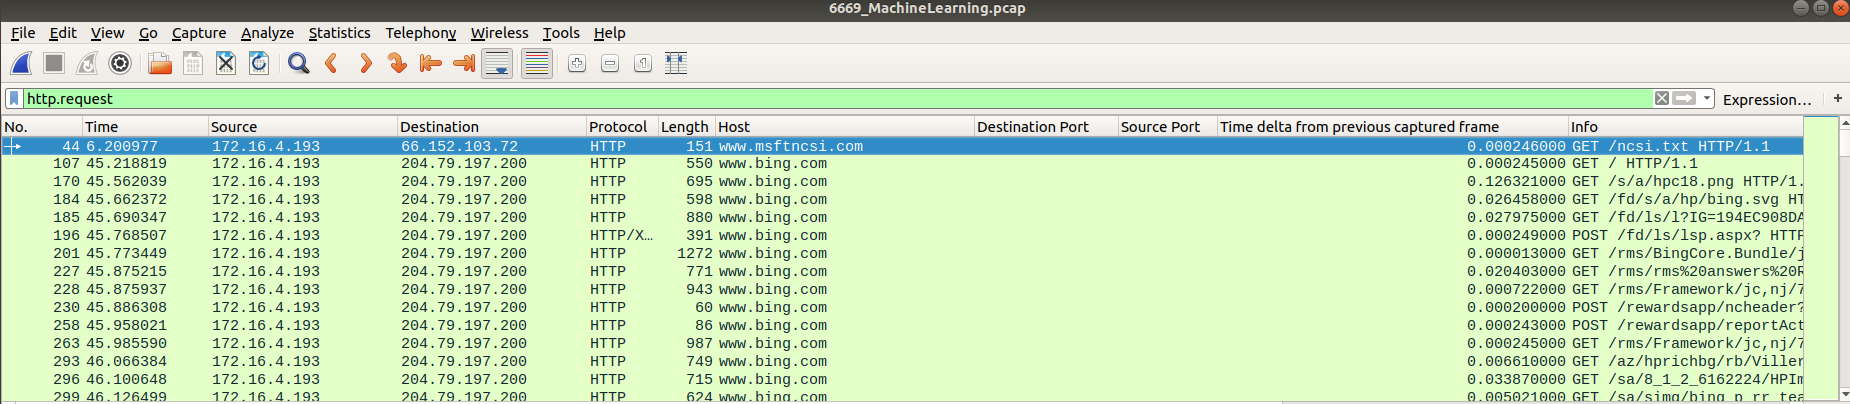
\includegraphics[scale=0.2]{Wireshark/2_1.png} 
\caption{}
\end{figure}

\medskip
Se encontraron sitios como los mostrados en la siguiente Figura junto con su cantidad de apariciones.

\medskip
\begin{figure}[!htp]
\centering
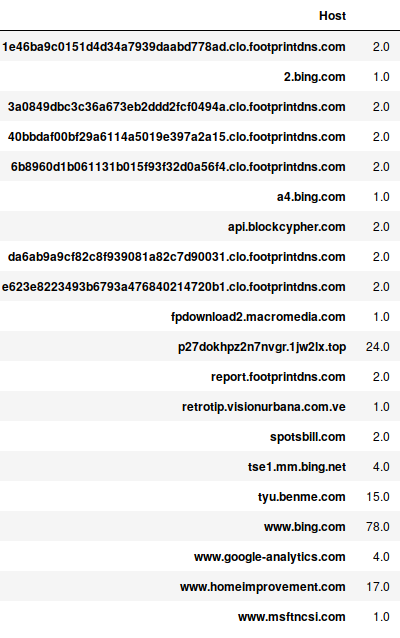
\includegraphics[scale=0.5]{Wireshark/Hosts.png} 
\caption{Lista de dominios generada con Python}
\end{figure}

Al observar estos dominios es importante la experiencia del analista, como primera medida verificamos las terminaciones, en la lista se identifica uno con final \textbf{.top}, googleando el dominio encontramos lo siguiente:
\newpage

\begin{figure}[!hp]
\centering
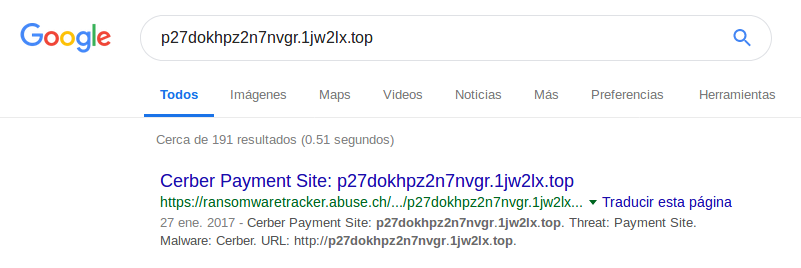
\includegraphics[scale=0.5]{Wireshark/google.png} 
\caption{}
\end{figure}

\medskip

Aquí se identifica el malware, el cual se trata de un \textbf{Ransomware}
 del tipo \textbf{Cerber}, conociendo esto se podría prohibir el tráfico a este sitio, sin embargo además de ser algo relativamente simple, no produce ningún tipo de solución ya que el virus podría cambiar de página, por ende queda pendiente encontrar algún comportamiento anómalo en el tráfico, de esta manera se continúa con el análisis utilizando un plugin de Wireshark llamado Snort, de aquí se pretende obtener alguna información del exploit utilizado e información de la IP de la cual este proviene.

\medskip
\begin{figure}[!htp]
\centering
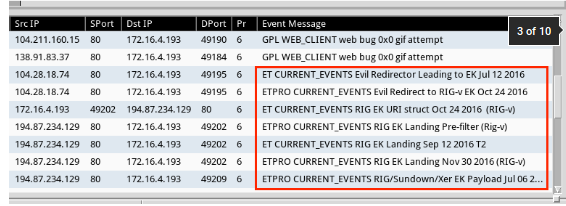
\includegraphics[scale=0.5]{Wireshark/Snort.png} 
\caption{}
\end{figure}
Acorde a lo investigado RIG Exploit Kit es unos de los más activos y utilizados actualmente para realizar este tipo de ataques, tomamos la ip 194.87.234.129 y procedemos a buscarla en el tráfico con Wireshark mediante el filtro
\medskip
\begin{figure}[!htp]
\centering
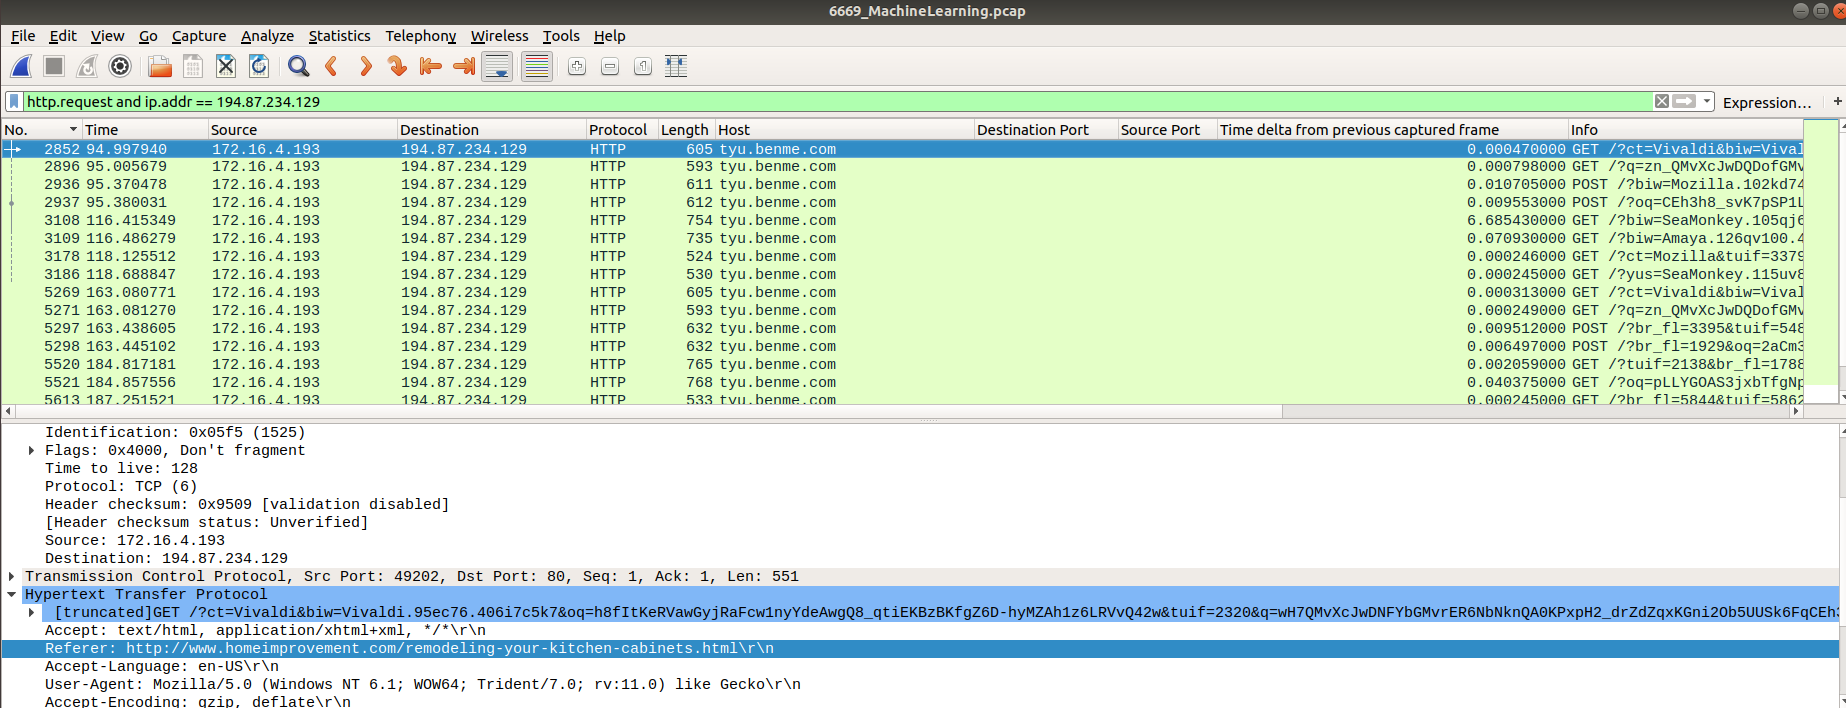
\includegraphics[scale=0.3]{Wireshark/5.png} 
\caption{}
\end{figure}


\medskip

\newpage
Como conclusion, entendemos que el exploit es injectado mediante el sitio www.homeimprovement.com el cual esta en el listado de la Figura 8.

\medskip

Finalmente en la siguiente imagen se pueden ver algunos paquetes correspondientes al tráfico generado durante la infección. A partir de la línea 3977 el comportamiento no sigue los patrones de tráfico habituales en una red. Se pueden observar paquetes UDP que en un breve intervalo de tiempo (menos de 1 segundo) \textbf{proceden de una misma IP de origen y que se dirige a diferentes (y en muchos casos consecutivas) IP de destino públicas}. Además, los puertos origen y destino son fijos.

\begin{figure}[!htp]
\centering
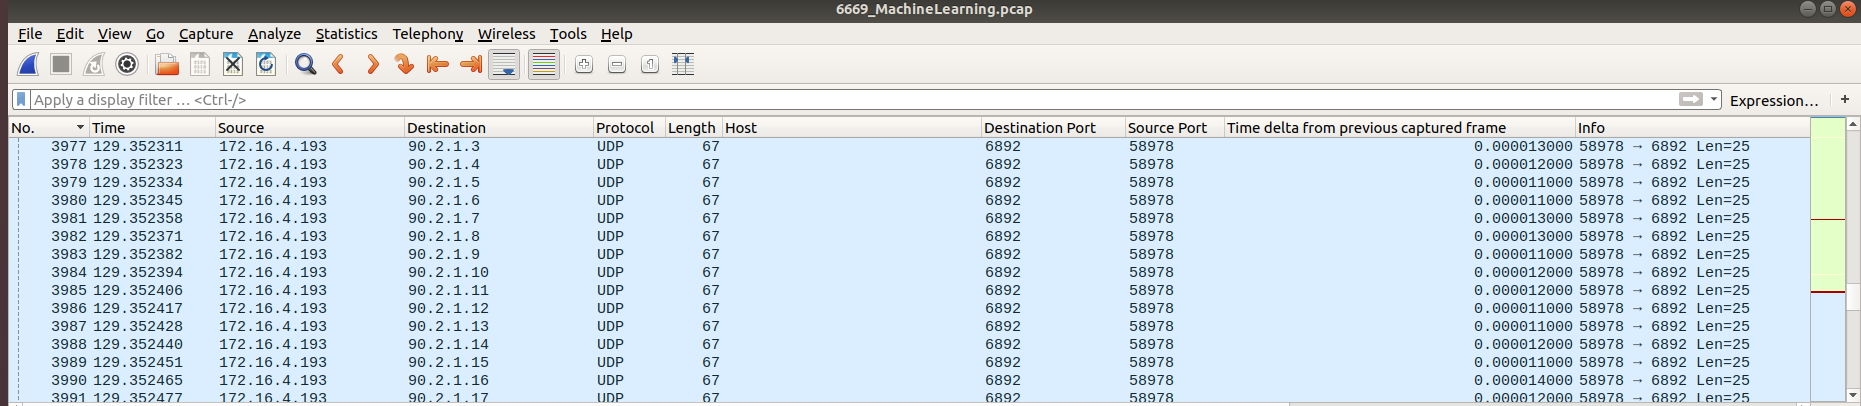
\includegraphics[scale=0.3]{Wireshark/6.png} 
\caption{}
\end{figure}

\medskip

Es este el cual se detecta cómo el comportamiento anómalo, el cual será trasladado al algoritmo de machine learning para que pueda prever este tipo de situaciones y notificarlo.

\medskip

\newpage
En conclusion del analisis del trafico:







\begin{table}[htbp]
\begin{center}
\begin{tabular}{|l|l|l|l|}
\hline
IP y Puerto & Sitio Web & Info \\
\hline
104.28.18.74 port 80  & www.homeimprovement.com & Sitio web comprometido  \\
139.59.160.143 port 80 & retrotip.visionurbana.com.ve & Puerta de rediccionamiento\\
194.87.234.129 port 80 & tyu.benme.com & Rig EK\\
198.105.121.50 port 80 & p27dokhpz2n7nvgr.1jw2lx.top & Cerber ransomware\\
90.2.1.0 to 90.2.1.31 (90.2.1.0/27) port 6892 & - & Cerber post-infection UDP traffic\\
90.3.1.0 to 90.3.1.31 (90.3.1.0/27) port 6892 & -  & Cerber post-infection UDP traffic\\
91.239.24.0 to 91.239.25.255 (91.239.24.0/23) port 6892 & - & Cerber post-infection
UDP traffic\\

\hline

\end{tabular}
\label{tabla:sencilla}
\end{center}
\end{table}


\subsection{Entrenamiento}

Basándose en esta simple observación definida anteriormente, se centra el funcionamiento del algoritmo en la creación de un feature o característica que cuenta el número de flujos en un intervalo de tiempo parametrizable en segundos, que desde una misma IP origen se conectan a diferentes IP destino públicas, con tráfico de un determinado protocolo y usando un cierto puerto destino. Lo que se espera es que para el tráfico normal este valor sea bajo y se consideran anomalías aquellos que tengan valores altos. Esto se trata tan sólo de un simple ejemplo y se podrían definir más características. De hecho, definir características acertadas (además de la adecuada elección del dataset) es el arte que puede llevar a que los algoritmos de aprendizaje sirvan realmente en el mundo real.\\

El primer desafío que se encontró en comparación del caso anterior, fue en la propia generación de los datos, esta vez solamente teníamos un archivo .pcap con el tráfico de red, el cual a su vez era escaso, ya que comentamos de la Figura, solo tenía 6033 líneas. De nuestro estudio en la temática sabemos lo importante que es tener datos de valor, y cuanto más grande sea el dataset aún mejor ya que brindarle más información al algoritmo implica más robustez y menos overfit, es decir, que la solución se vuelva muy particular y deje de generalizar para otro tipo de casos, lo cual queremos evitar. Por ende para ampliar el set de datos, se tomaron otros ejemplos de tráfico de ransomware, donde se detectó que el patrón seguía siendo el mismo, a su vez tener en el mismo dataset infecciones de fechas temporales distintas, con IPs (origen y destino) distintas de ataque, e incluso puertos distintos resulta valioso.\\

A su vez también debemos brindarle a este información de tráfico que sea “normal” sin malware, el cual es extremadamente útil para enfatizar cuando existe o no una anomalía, para generarlo lo hicimos con una de los propias computadoras de los integrantes del grupo capturando paquetes mediante Wireshark.\\


\medskip

Realizado esto se prosiguió generando un dataframe que tenga el contenido de toda la información recolectada, para eso utilizamos \textbf{pandas} la cual es una librería de python para el análisis y creación de estructuras de datos, herramienta muy utilizada en el ámbito de machine learning. \\

A continuación, se creó un nuevo feature (columna) para categorizar al tráfico si este era como un ataque o como normal, esto fue realizado teniendo en cuenta todo el análisis explicado anteriormente. Este es muy necesario ya que será nuestro parámetro para más tarde establecer las comparaciones con las predicciones que hagamos a partir de nuestro entrenamiento con \textbf{Random Forest}.\\

\medskip
El segundo paso fundamental para resolver el problema, fue trabajar la creación de un nuevo dataframe que contenga la información de valor en términos de flujos de datos, por esta razón es esencial el preprocesamiento del dataset, ya que cuando el algoritmo fue entrenado sin procesamiento alguno las predicciones acertadas fueron muy bajas. Para esto se decidio agrupar bajo las siguientes condiciones, las cuales fueron detectadas con el análisis del Ransomware:
\begin{itemize}
\item Por tiempo, estimado en 1 segundo, esta parámetro puede ser variable para obtener resultado distintos, encontramos que una gran cantidad de paquetes UDP fueron enviados en este lapso de tiempo 
\item Por IP origen, se encontró un comportamiento anómalo cuando la IP source se mantenía constante pero la IP destino era cambiante en un breve lapso de tiempo, el cual es cuando actuaba Cerber.
\item Por puertos, durante el ataque los puertos se mantenían constantes.
\end{itemize}

\begin{figure}[!htp]
\centering
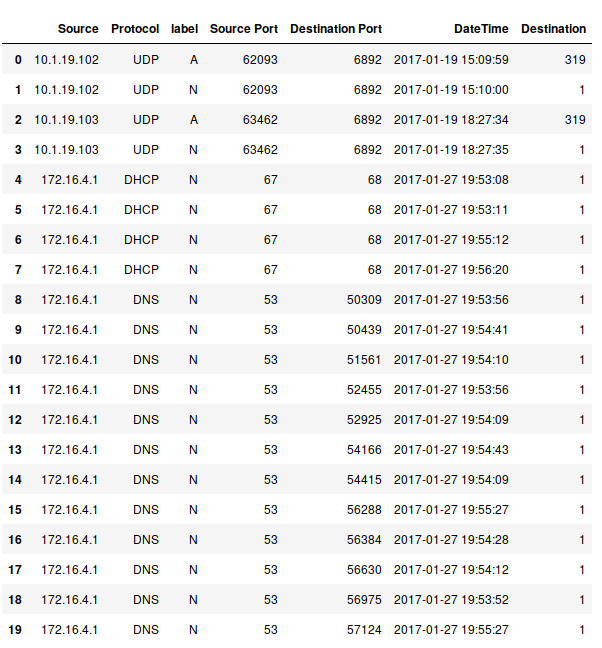
\includegraphics[scale=0.5]{Wireshark/magicmike.png} 
\caption{}
\end{figure}



%%%%%%%%%
\newpage
%%%%%%%%%



A continuación una serie de ejemplos de árboles de decisión generados por nuestro programa:
\begin{figure}[!hbp]
\begin{subfigure}{.5\textwidth}
  \centering
  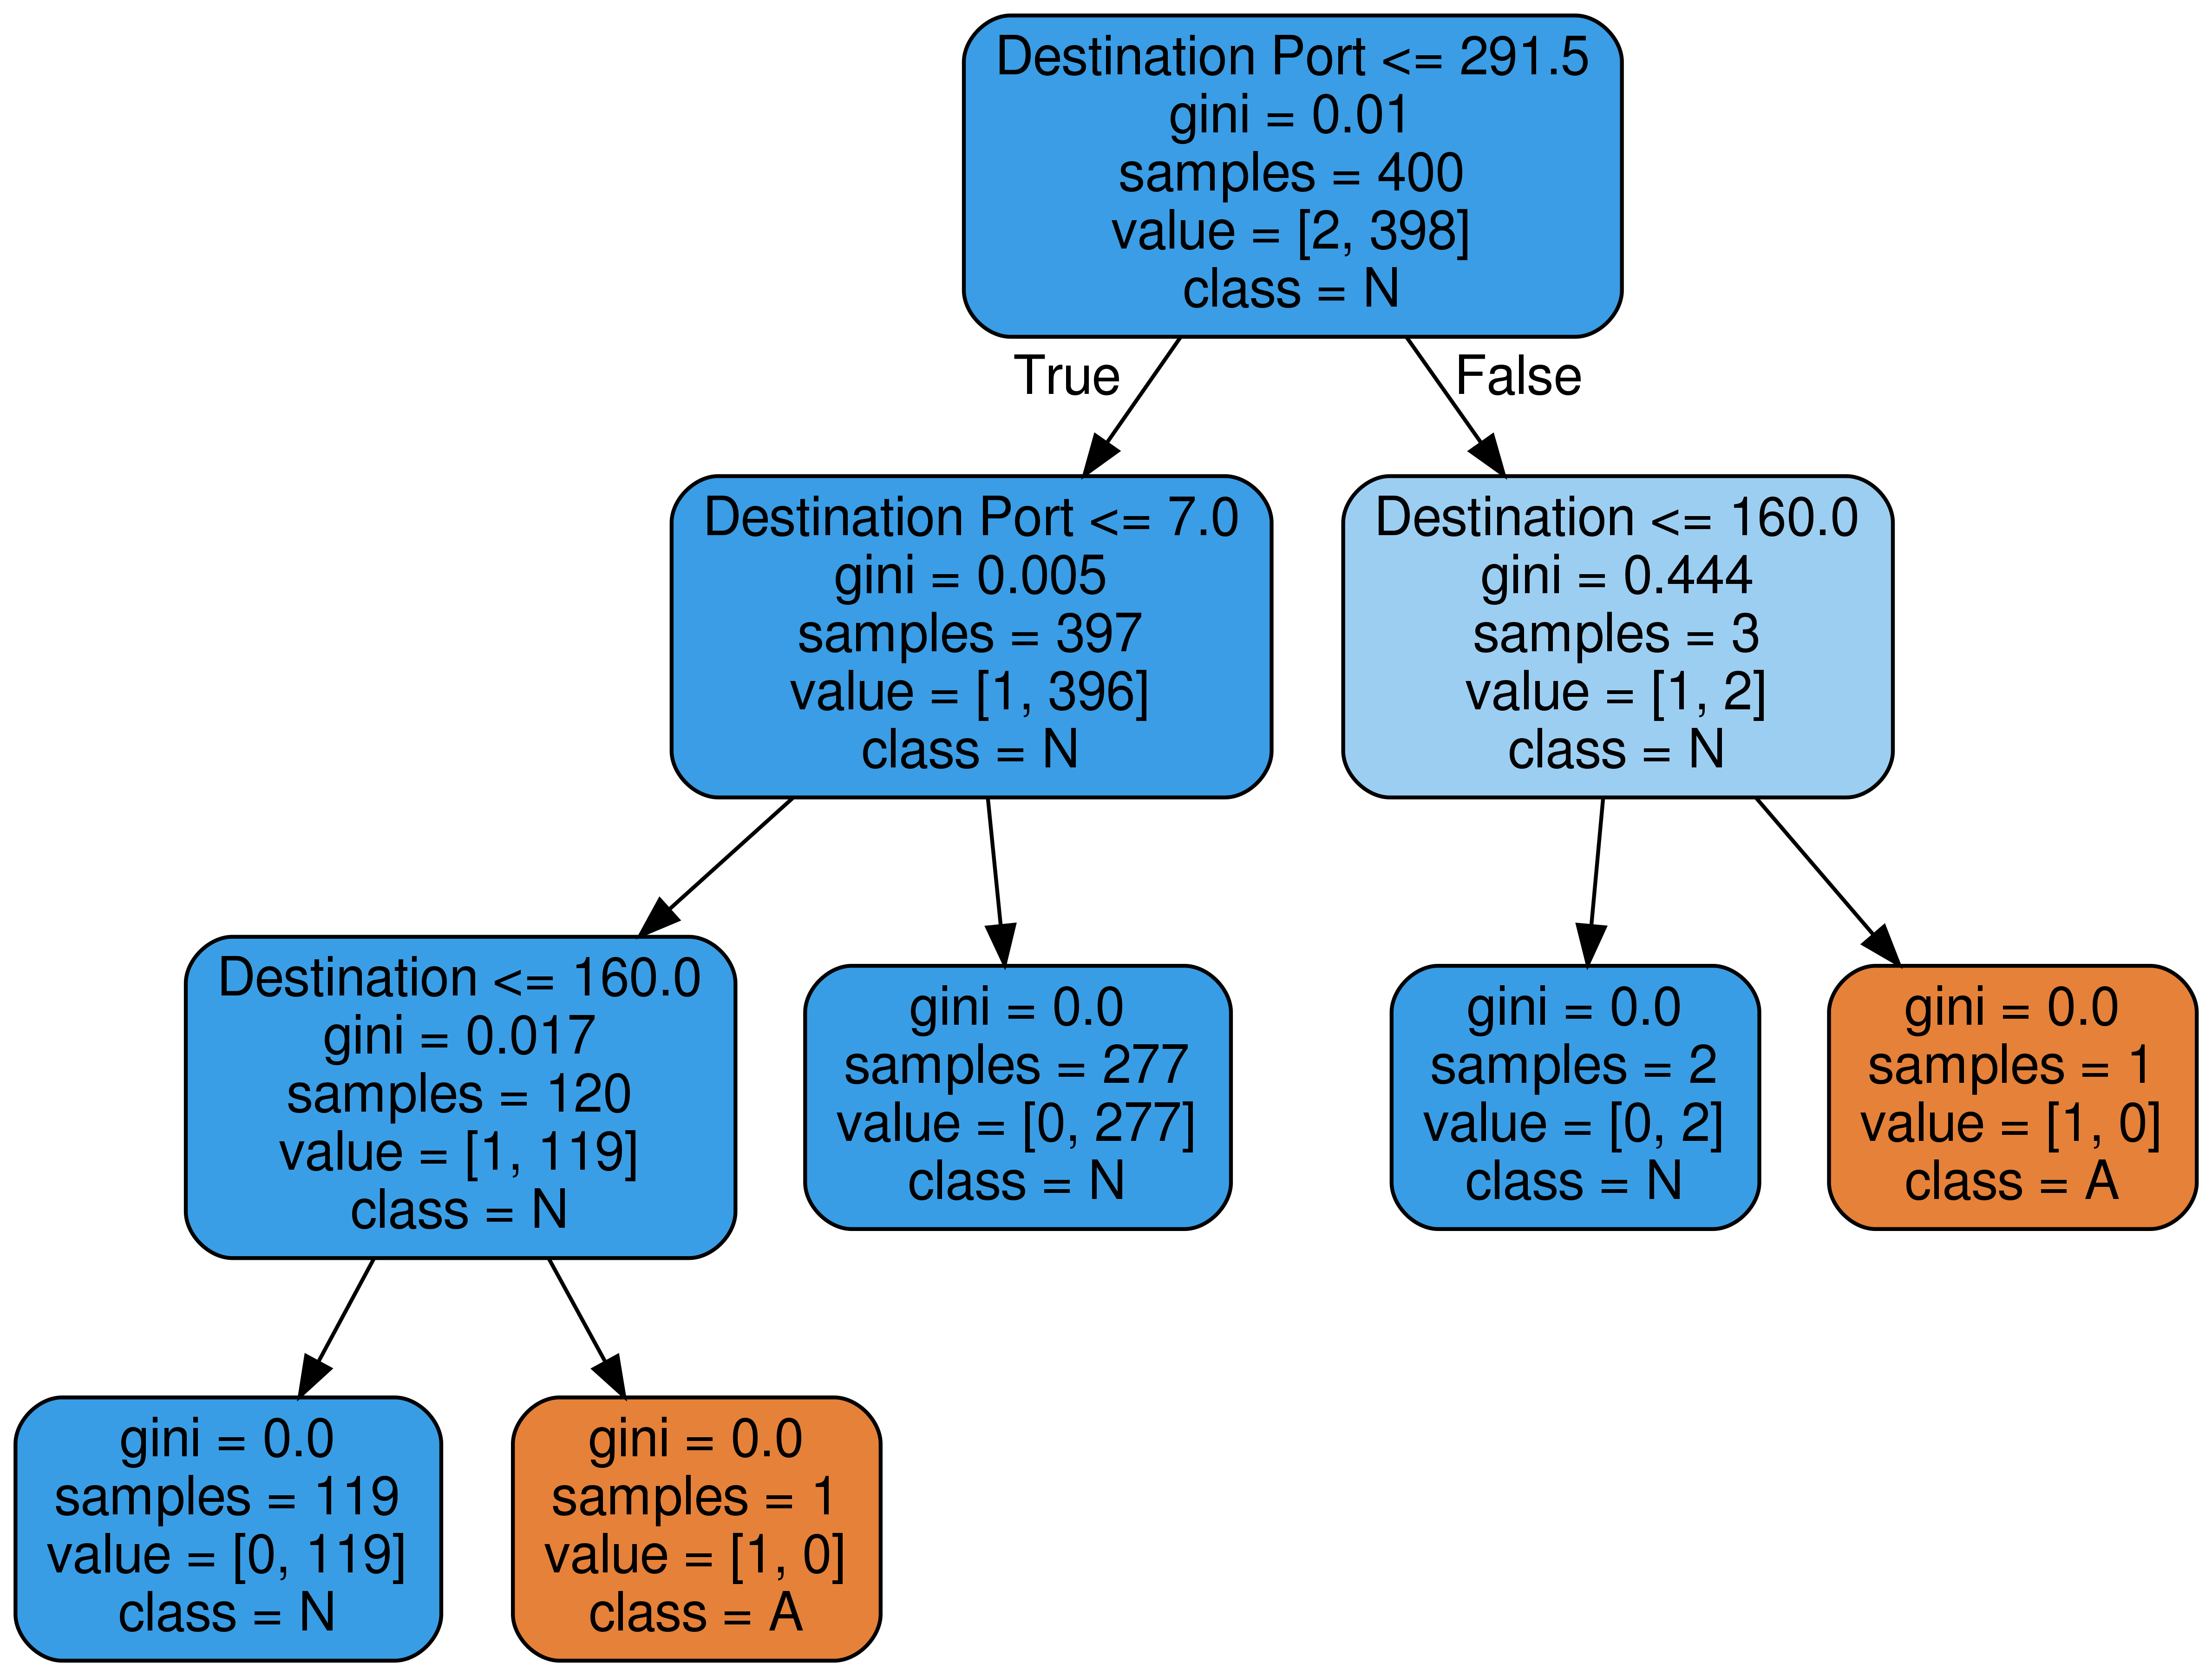
\includegraphics[width=.8\linewidth]{Wireshark/Tres/1.png}
  \caption{}
  \label{fig:sfig1}
\end{subfigure}%
\begin{subfigure}{.5\textwidth}
  \centering
  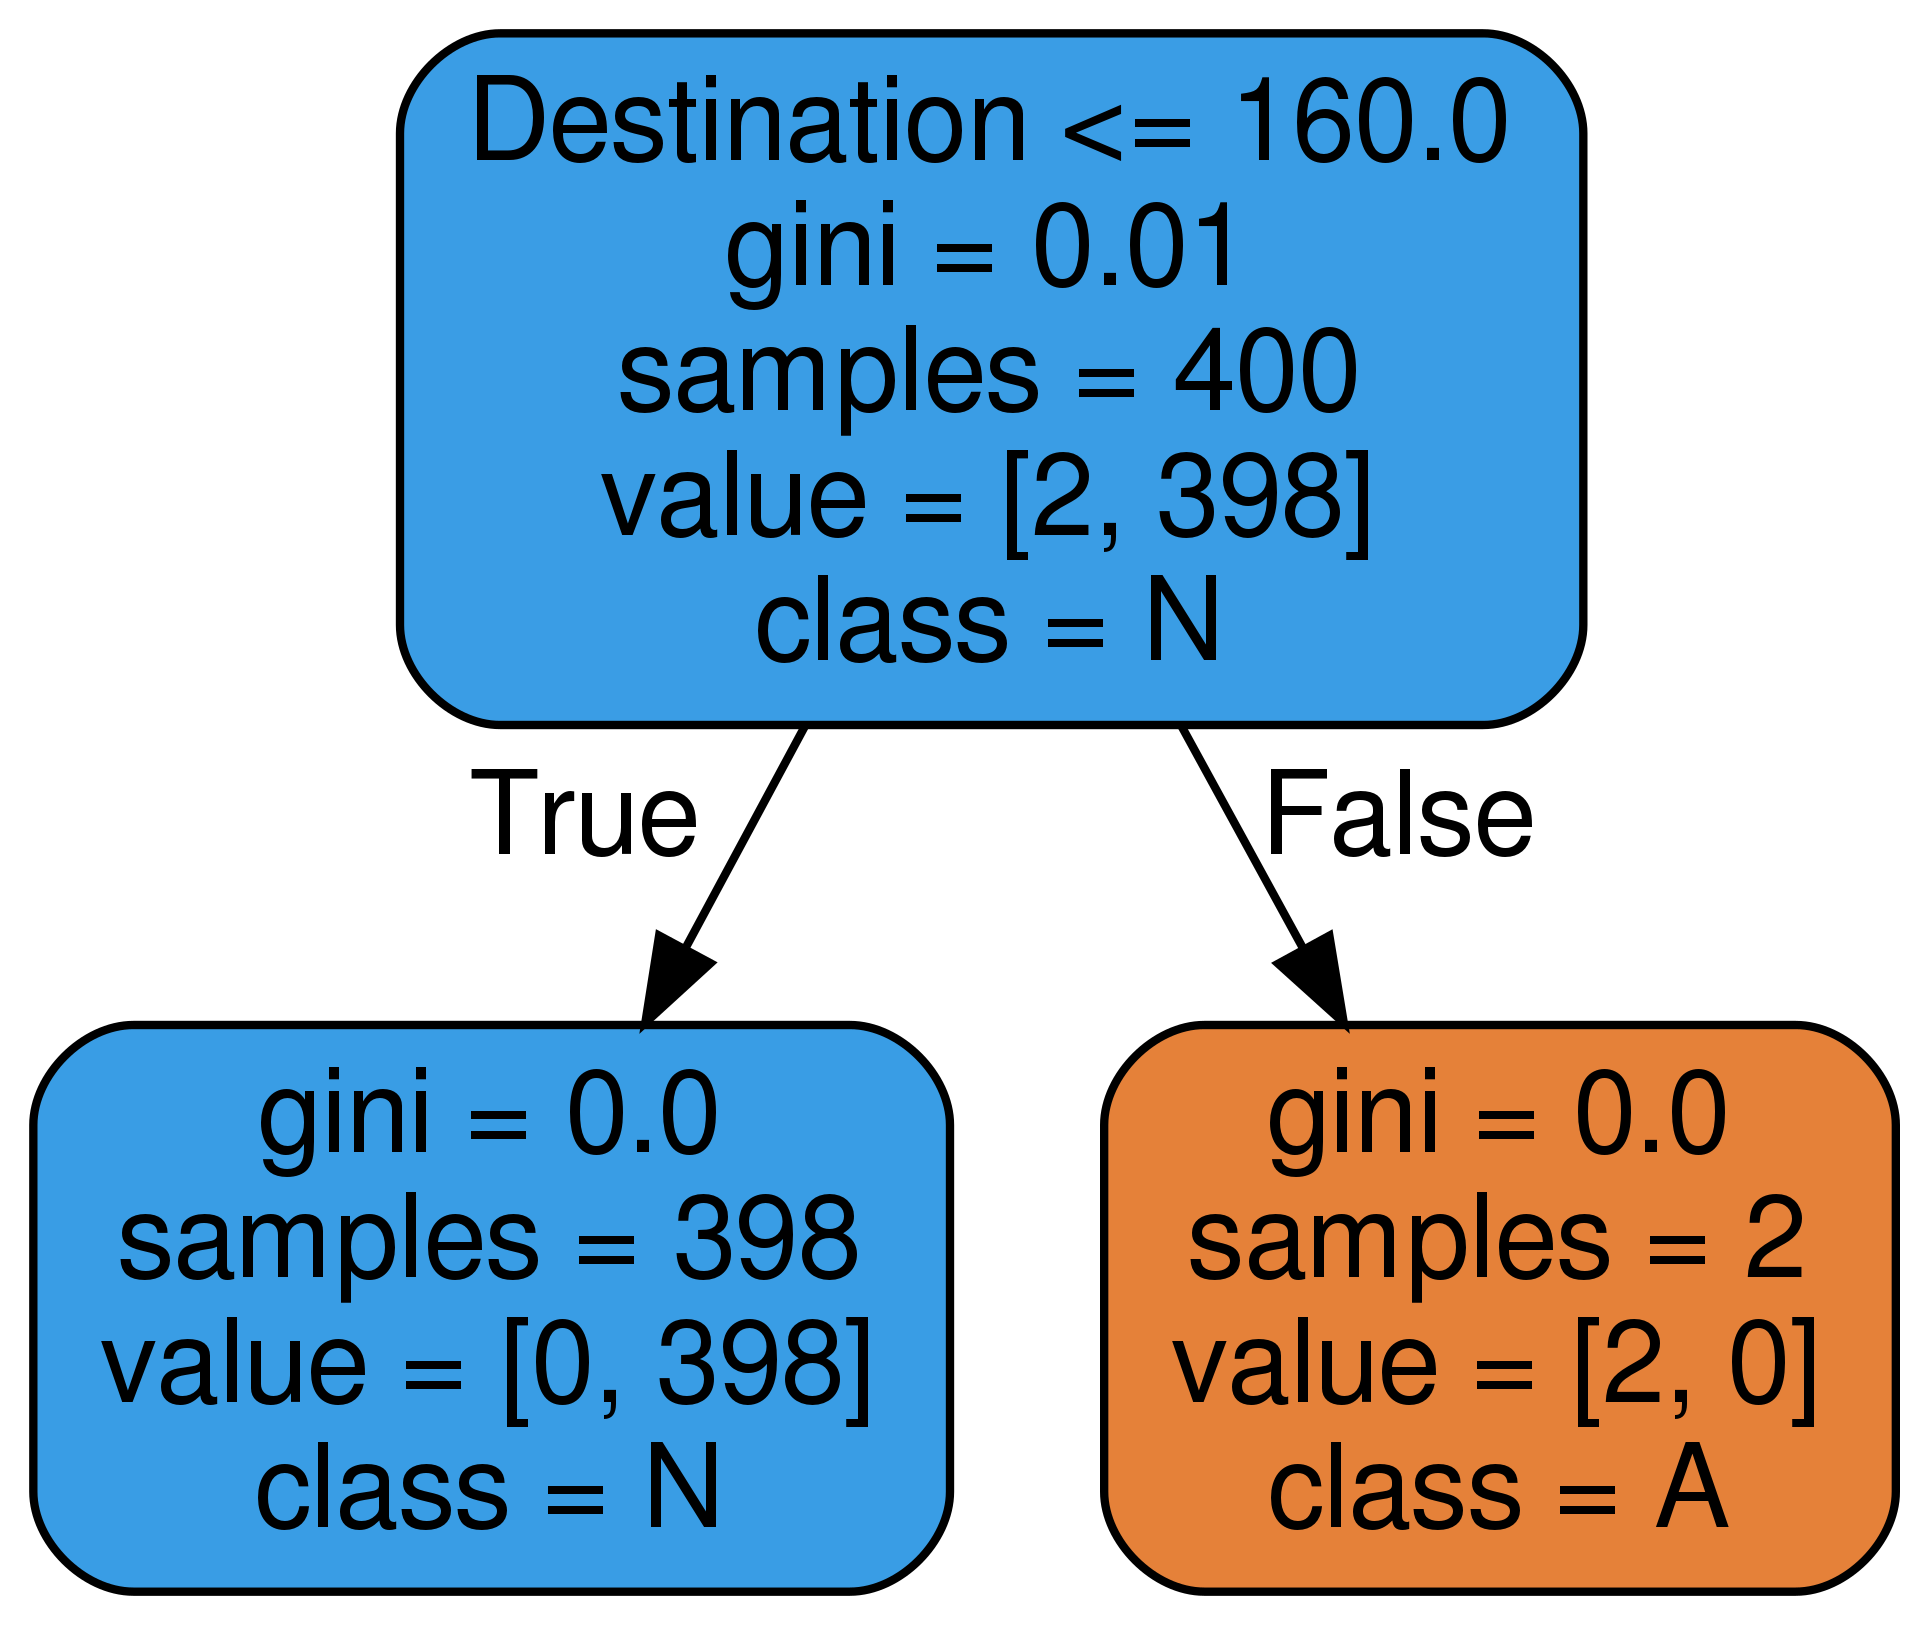
\includegraphics[width=.8\linewidth]{Wireshark/Tres/2.png}
  \caption{}
  \label{fig:sfig2}
\end{subfigure}
\begin{subfigure}{.5\textwidth}
  \centering
  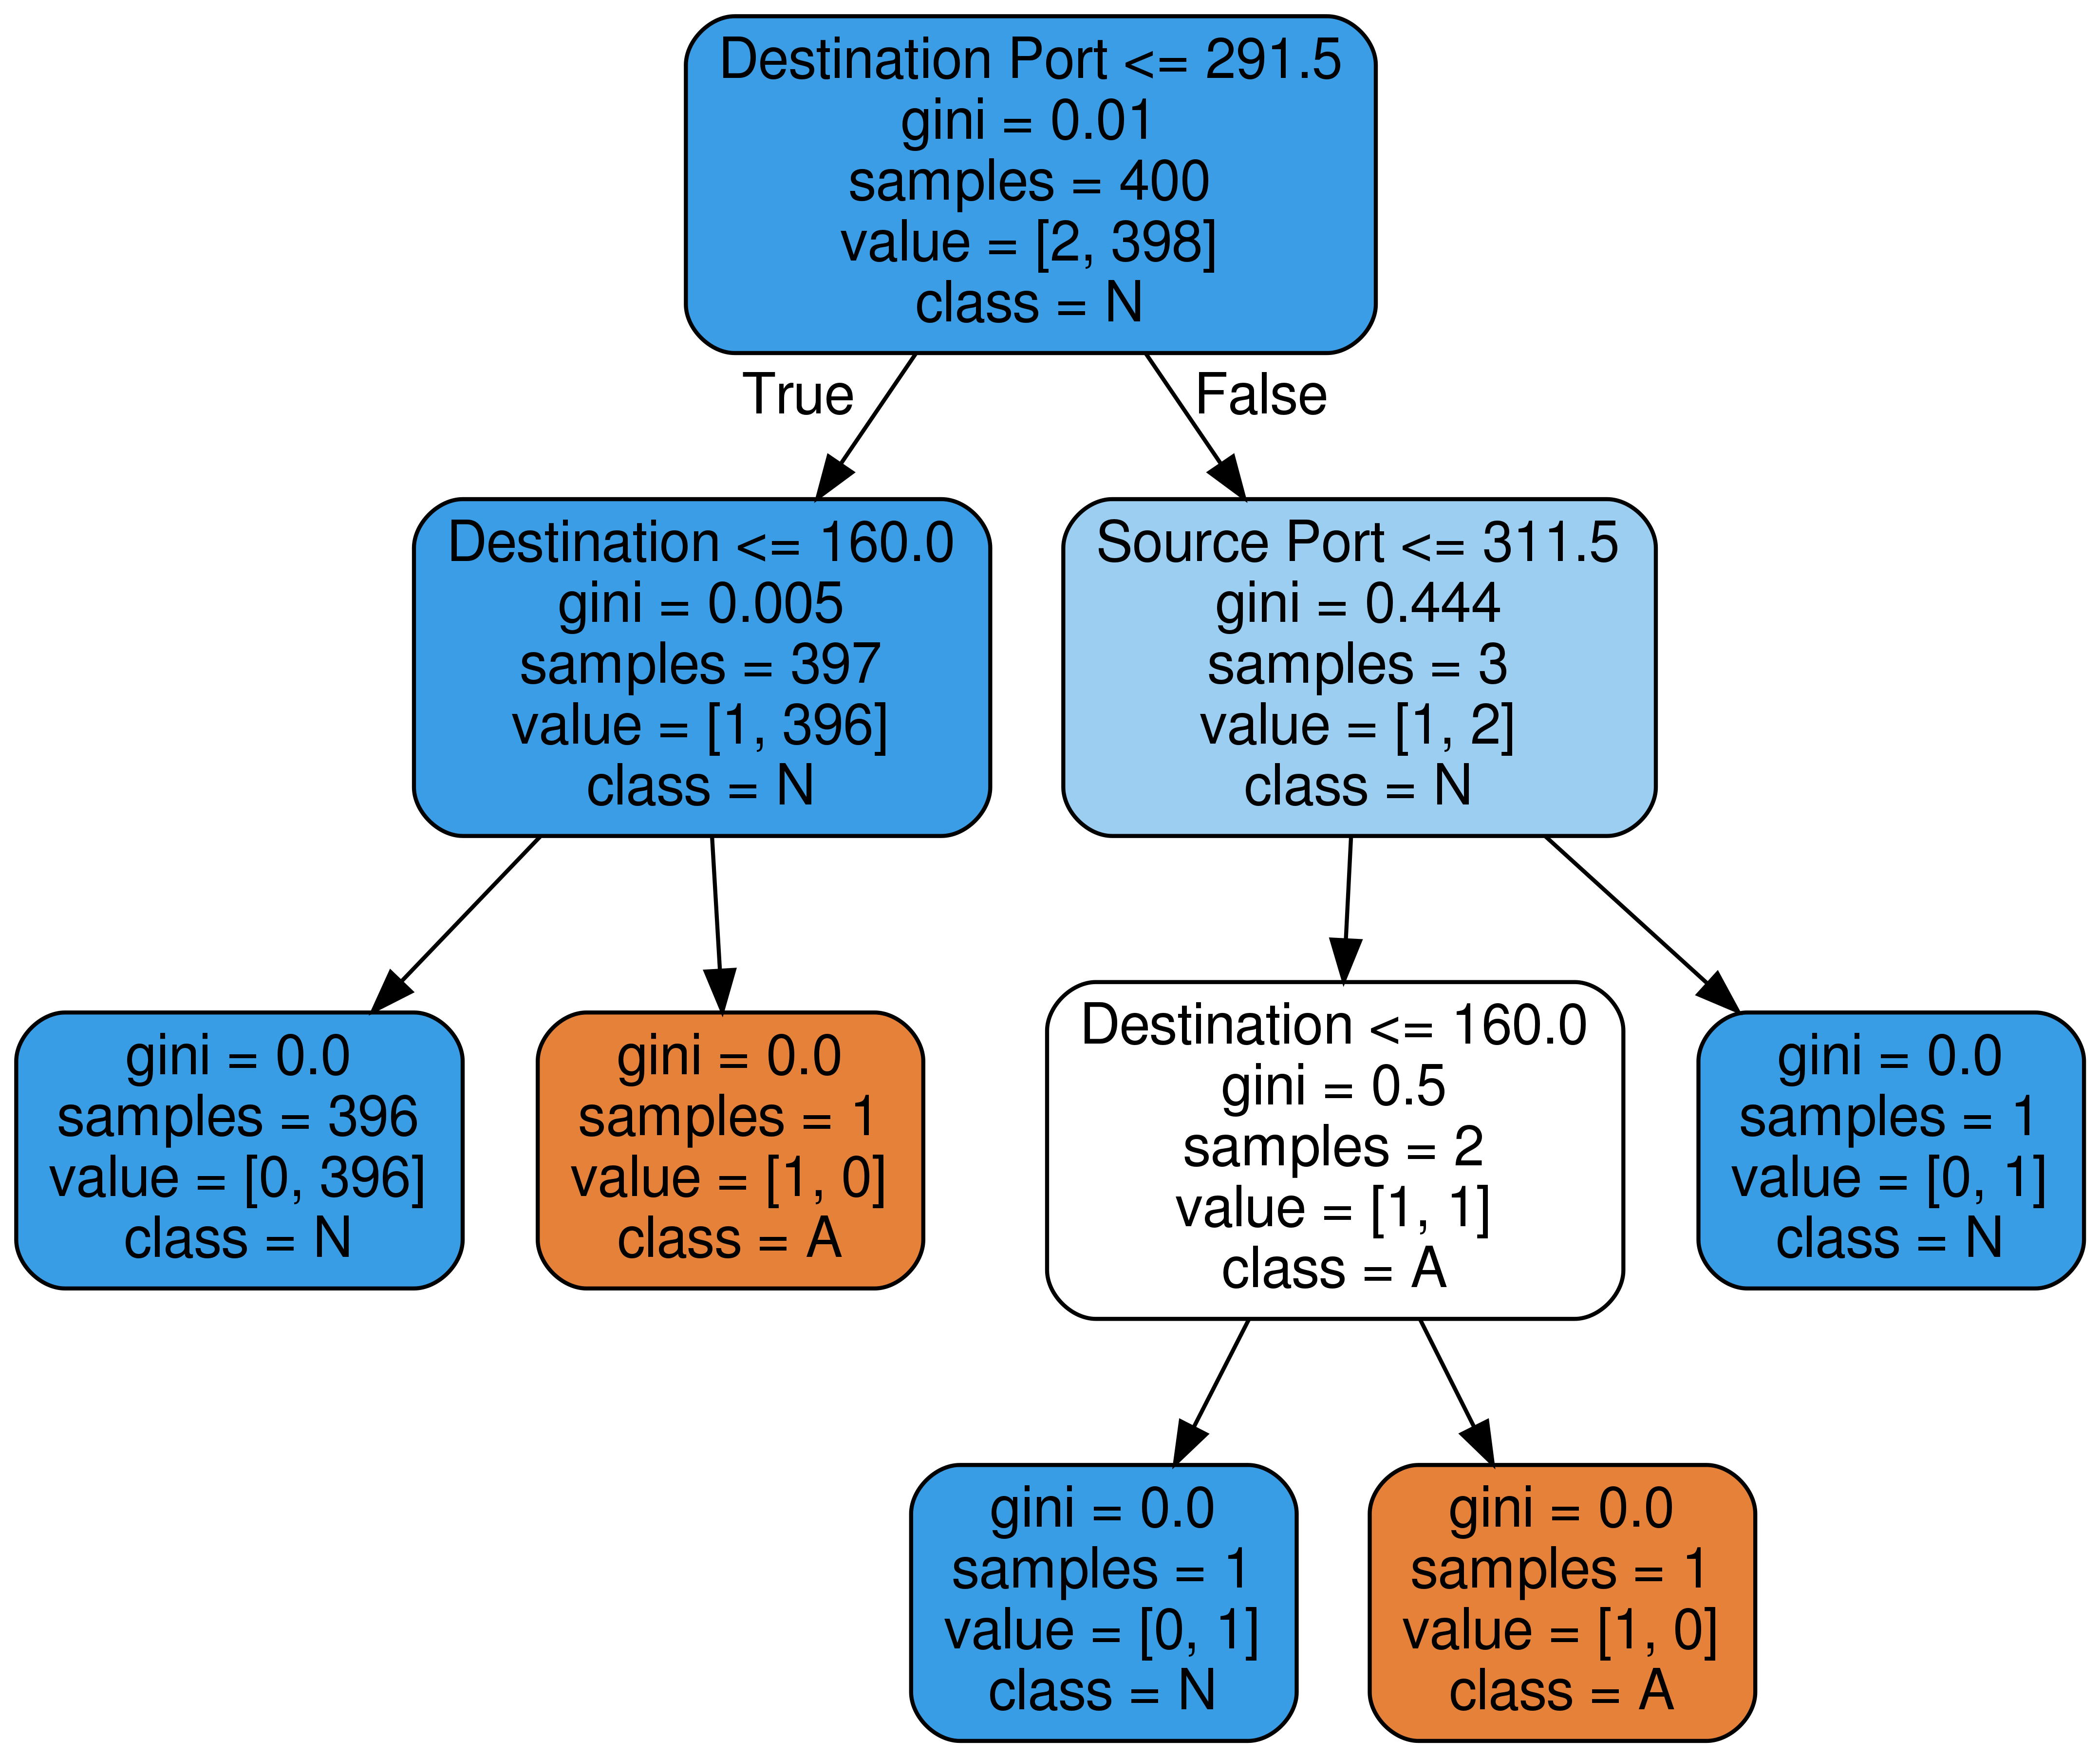
\includegraphics[width=.8\linewidth]{Wireshark/Tres/3.png}
  \caption{}
  \label{fig:sfig2}
\end{subfigure}
\begin{subfigure}{.5\textwidth}
  \centering
  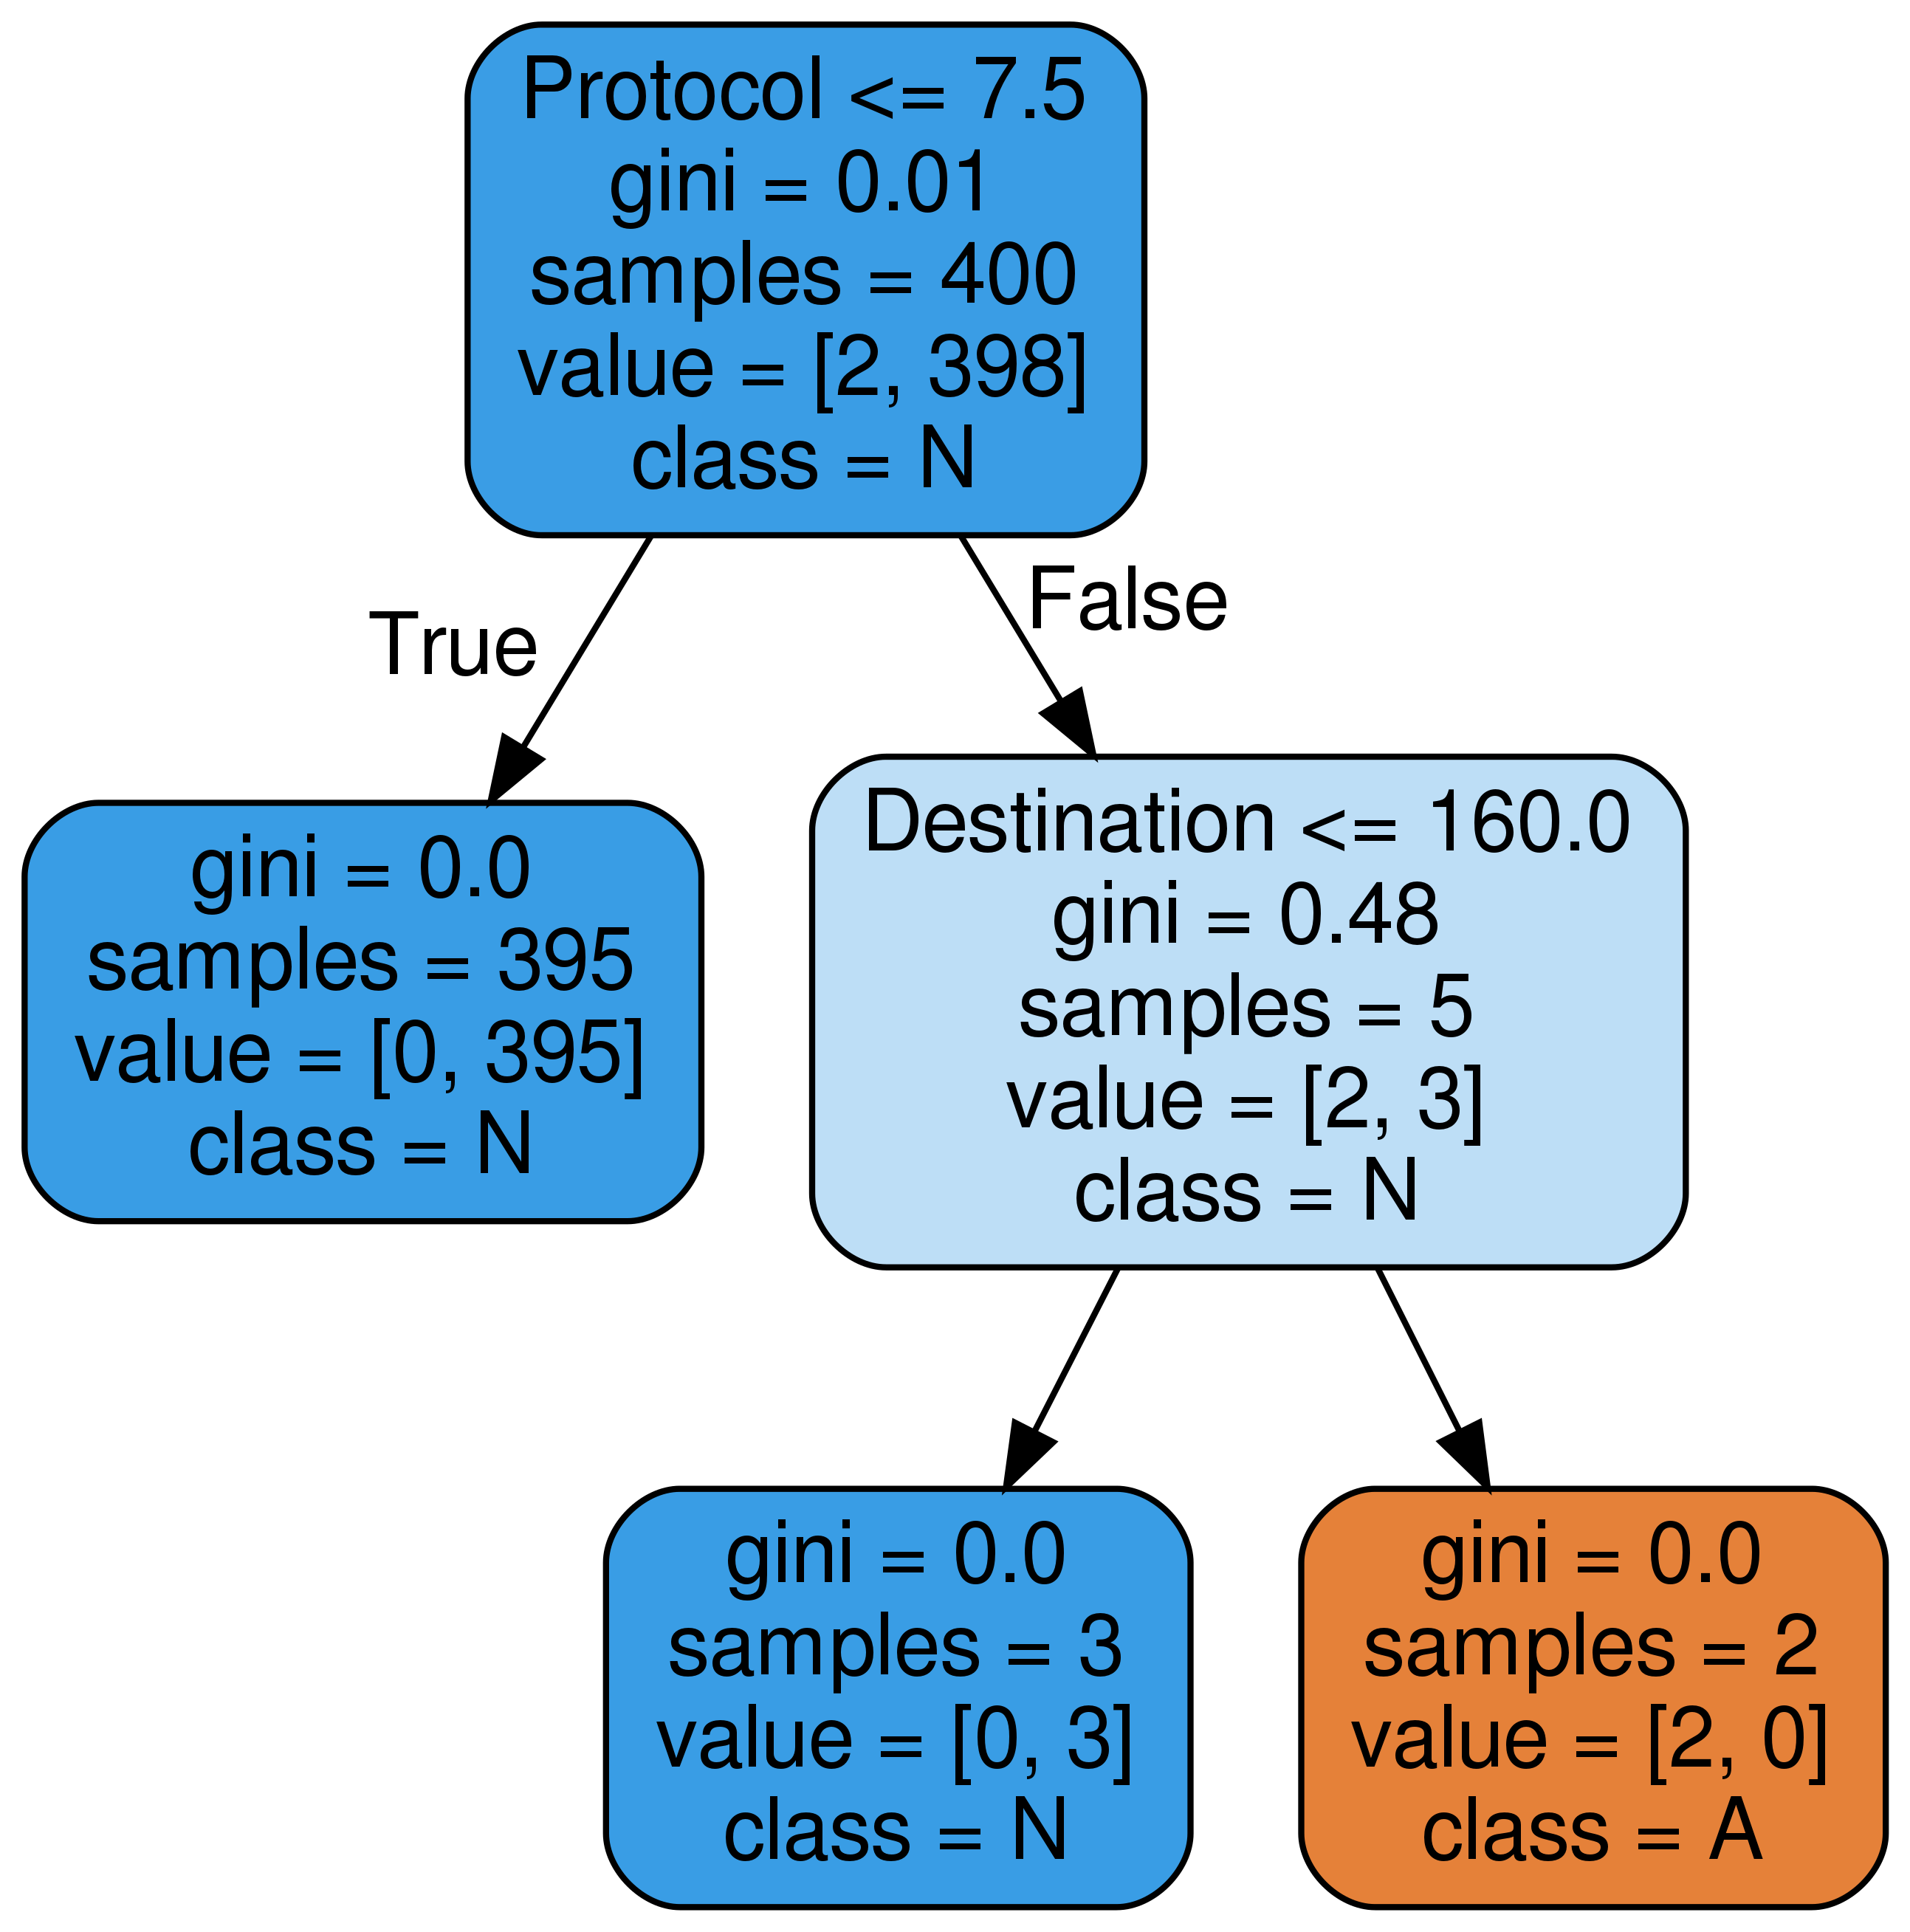
\includegraphics[width=.8\linewidth]{Wireshark/Tres/4.png}
  \caption{}
  \label{fig:sfig2}
\end{subfigure}
\begin{subfigure}{.5\textwidth}
  \centering
  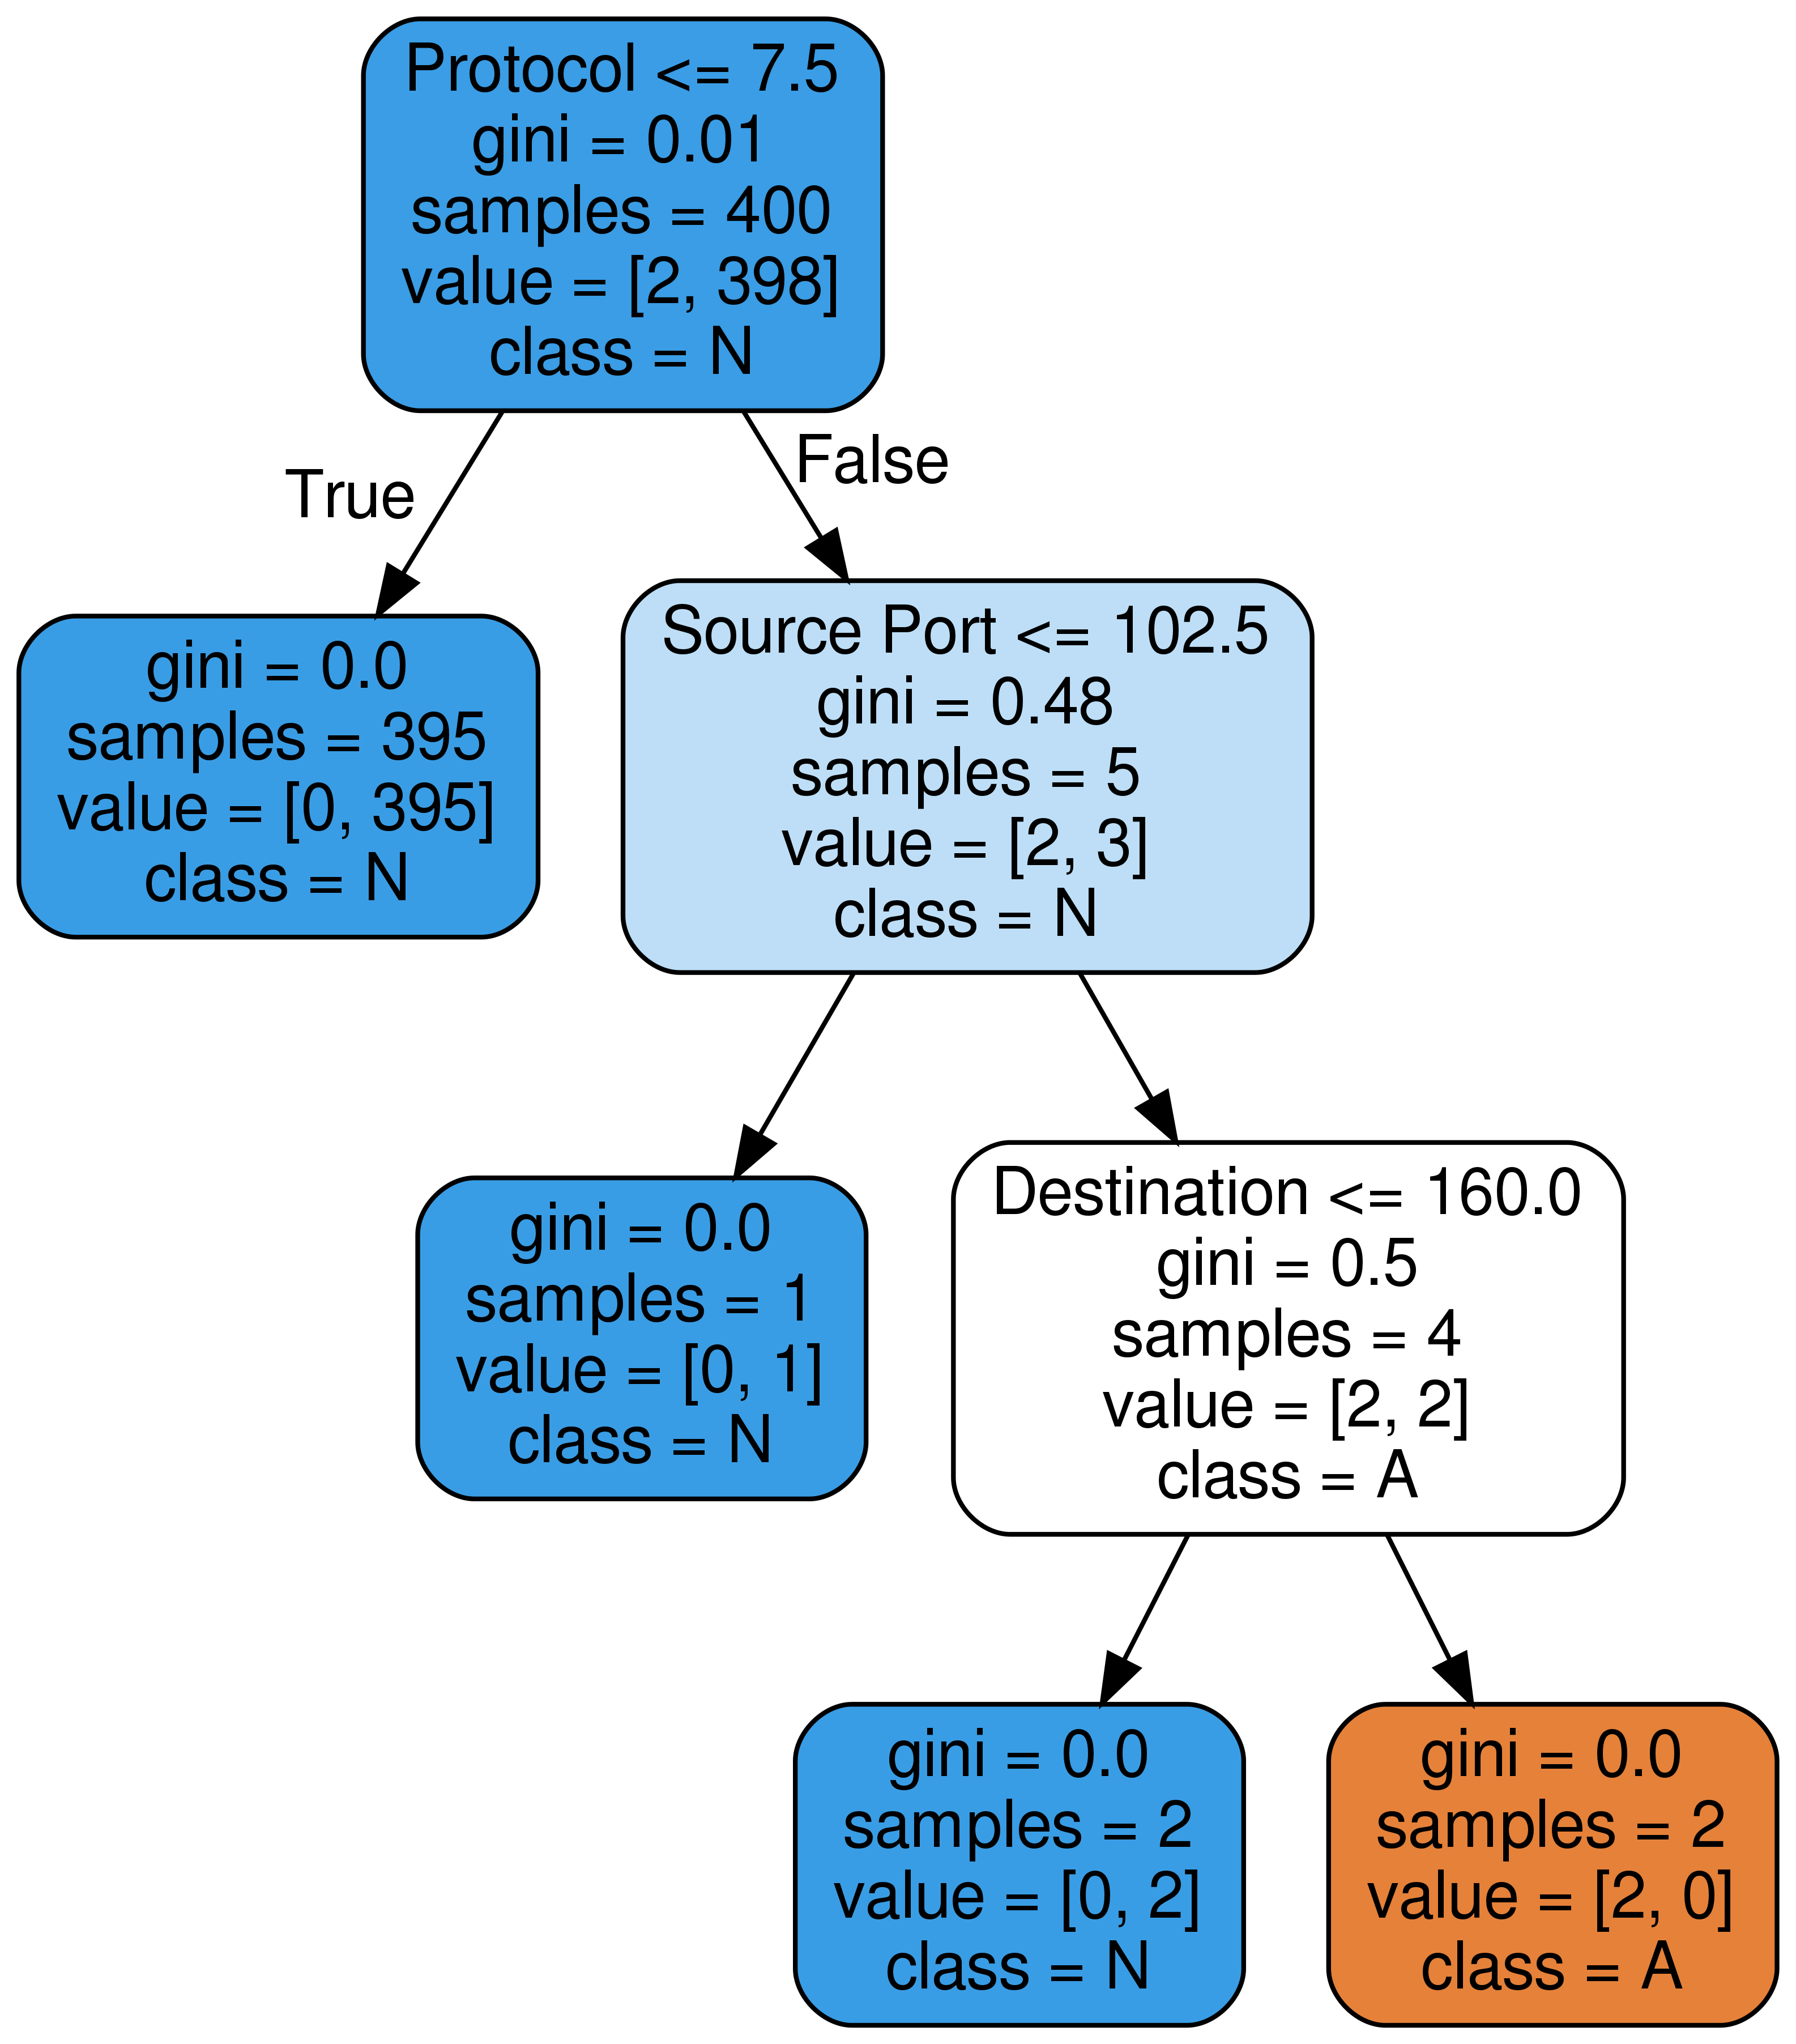
\includegraphics[width=.8\linewidth]{Wireshark/Tres/5.png}
  \caption{}
  \label{fig:sfig2}
\end{subfigure}
\begin{subfigure}{.5\textwidth}
  \centering
  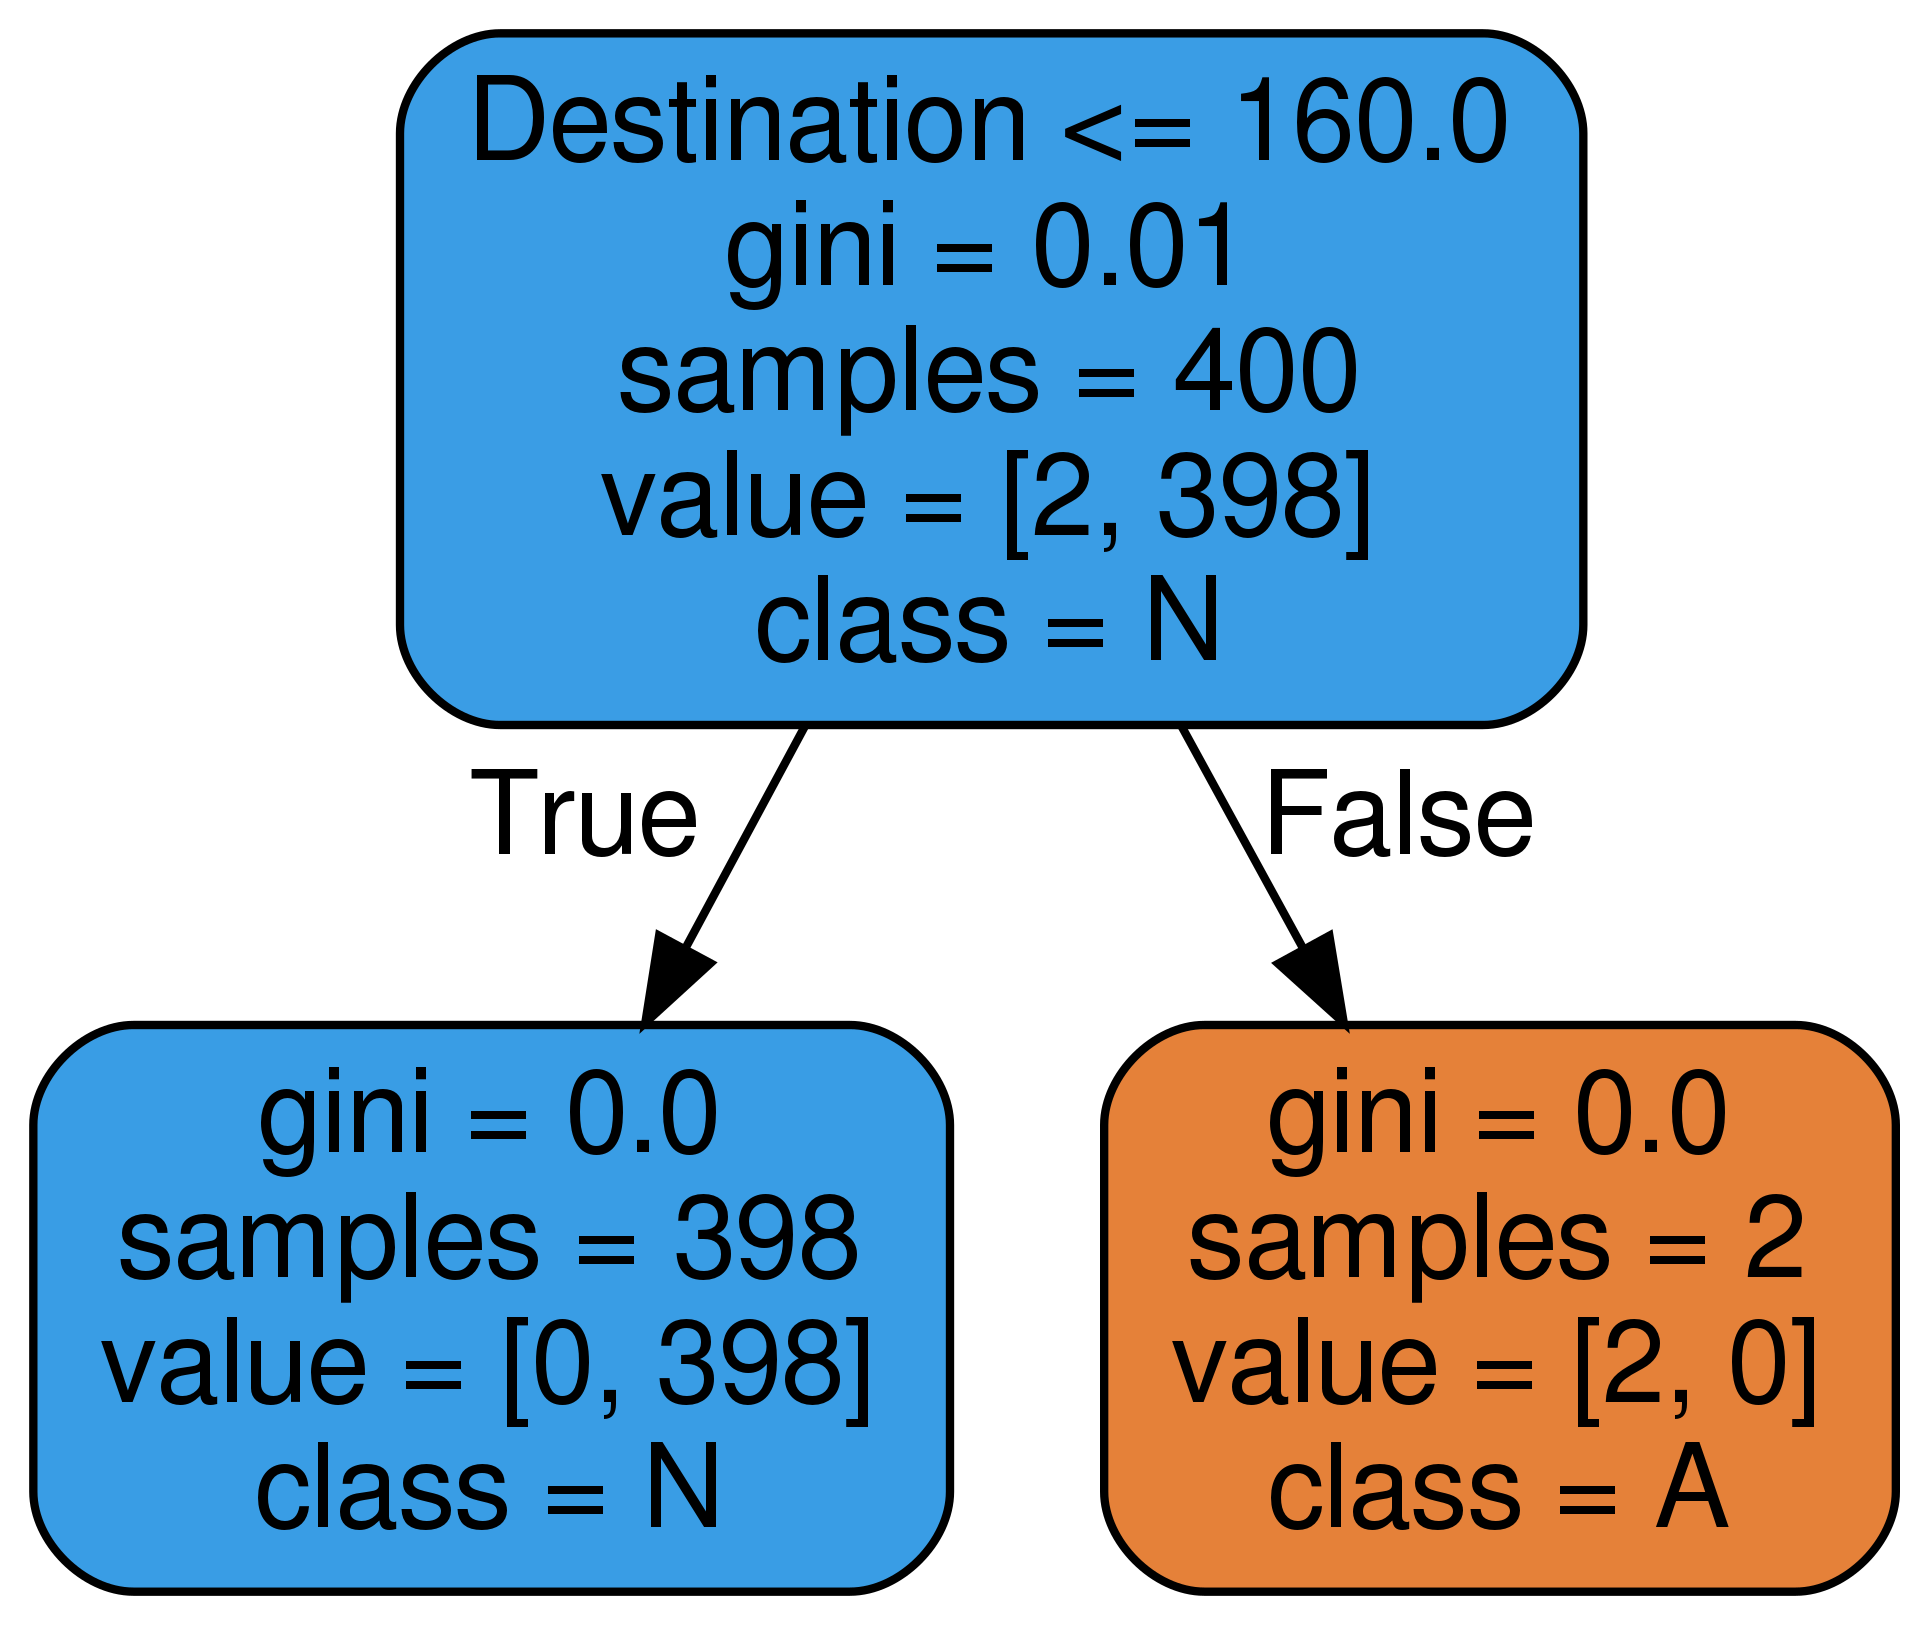
\includegraphics[width=.8\linewidth]{Wireshark/Tres/6.png}
  \caption{}
  \label{fig:sfig2}
\end{subfigure}

\caption{Arboles de decision}
\label{fig:fig}
\end{figure}

Finalmente se logró clasificar por medio de este algoritmo a los datos con una precisión del \textbf{0.9925373134328358}

\medskip

\normalsize Para probar estos resultados se dividió nuestro set de datos en 60\% de entrenamiento y 40\% de prueba. Donde se encontró que las anomalías fueron detectadas todas correctamente lo cual era el objetivo principal de nuestro problema.

\section{Repositorio}
Link al repositorio: \textbf{https://github.com/AugustoArturi/Anomalias}

Archivos:
\begin{itemize}
\item{Detail\_ML\_Solution.ipynb, \textbf{caso 1}}
\item{Ransomware.ipynb, \textbf{caso 2}}
\end{itemize}

\section{Conclusion}

Los algoritmos de machine learning pueden ser herramientas muy utiles para utilizar en el area de seguridad informatica. En este trabajo se demostro que estos algoritmos pueden servir para detectar ataques que afectan a la disponibilidad del servicio (DOS), como tambien para los que afectan la integridad de los datos (Ransomware). Queda para futuros trabajos investigar en que otros pilares de la seguridad informatica se pueden usar estas herramientas.
\newpage





\begin{thebibliography}{9}
\bibitem{latexcompanion}  http://www.malware-traffic-analysis.net/.
\bibitem {latexcompanion} https://scikit-learn.org/

\bibitem {latexcompanion} https://www.stat.berkeley.edu/\~breiman/RandomForests/cc\_home.html

\bibitem {latexcompanion} https://kdd.ics.uci.edu/databases/kddcup99/task.html


\bibitem {latexcompanion} Apunte Luis Argerich 75.06 Organizacion de Datos - FIUBA
\end{thebibliography}

\end{document}

\begin{table}[htbp]
\begin{center}
\begin{tabular}{|l|l|l|l|}
\hline
Relacion & CK & PK & FK\\
\hline
A(idA,a1) & idA & idA & - \\
B(idB,b1) & idB & idB & -\\
D(idD,d1) & idD & idD & -\\
C(idC,c1) & idC & idC & -\\
E(idC,e1,e2) & idC & idC & idC\\
F(idC,f1,f2) & idC & idC & idC\\
R1(idC(1),idC(2)) & idC(1) , idC(2) & idC(1) & idC(1) , idC(2)\\
R2(idC(E),idD,r1) & {idC(E),idD} & {idC(E),idD} & idC(E) , idD\\ 
R3(idA,idB,idD) & $\left\lbrace idA,idB \right\rbrace$ , $\left\lbrace idA, idD\right\rbrace$, $\left\lbrace idB, idD \right\rbrace$ &  $\left\lbrace idA,idB \right\rbrace$ & idA , idB , idD\\
\hline

\end{tabular}
\label{tabla:sencilla}
\end{center}
\end{table}

\section{Cosas}

\textbf{Sistema Operativo}

\begin{itemize}

\item \textbf{Play referee}: manejar los recursos compartidos entre 

\begin{itemize}
\item Resource Allocation: 
\item Communication: 
\end{itemize}


\item \textbf{Play illusionist}:
\item \textbf{Provide glue}: 
\end{itemize}

\begin{figure}[!htp]
\centering
\includegraphics[scale=0.4]{SisopPC}
\caption{Capas de la PC}
\end{figure}

$T_{avg} = \dfrac{T_{turnaroundA} + T_{turnaroundB} + T_{turnaroundC}}{3}$\\



$T_{avg} = \dfrac{10 + 20 + 30}{3} = 20$\\



Ahora, dejemos de suponer que todos los procesos tardan lo mismo.

\begin{figure}[!ht]
\centering
{\includegraphics[scale=0.7]{fifo2}}
\label{fifo2}
  \caption{Politica FIFO: caso 2}
 
\end{figure}




$T_{avg} = \dfrac{T_{turnaroundA} + T_{turnaroundB} + T_{turnaroundC}}{3}$\\



$T_{avg} = \dfrac{100 + 110 + 120}{3} = 110$\\


\begin{figure}[!ht]
\begin{center}
  \subfigure[Llegada y largo de procesos]
  {\includegraphics[scale = 0.7]{rr1}}\hspace{10mm}
  \subfigure[Aplicacion de RR]{\includegraphics[scale = 0.7]{rr2}}
  \caption{Ejemplo de Round Robin}
\end{center}
\end{figure}


\lstset{language=C, breaklines=true, basicstyle=\footnotesize}
\begin{lstlisting}[frame=single]
include<pthread.h>
int pthread_create(pthread_t * thread, const pthread_att_t * att, void * (start_routine) (void *), void * arg)
\end{lstlisting}

\end{document}